%%%%%%%%%%%%%%%%%%%%%%%%%%%%%%%%%%%%%%%%%%%%%%%%%%%%%%%%%%%%%%%%%%%%
%% I, the copyright holder of this work, release this work into the
%% public domain. This applies worldwide. In some countries this may
%% not be legally possible; if so: I grant anyone the right to use
%% this work for any purpose, without any conditions, unless such
%% conditions are required by law.
%%%%%%%%%%%%%%%%%%%%%%%%%%%%%%%%%%%%%%%%%%%%%%%%%%%%%%%%%%%%%%%%%%%%

\documentclass[
  digital,     %% The `digital` option enables the default options for the
               %% digital version of a document. Replace with `printed`
               %% to enable the default options for the printed version
               %% of a document.
%%  color,       %% Uncomment these lines (by removing the %% at the
%%               %% beginning) to use color in the printed version of your
%%               %% document
  oneside,     %% The `oneside` option enables one-sided typesetting,
               %% which is preferred if you are only going to submit a
               %% digital version of your thesis. Replace with `twoside`
               %% for double-sided typesetting if you are planning to
               %% also print your thesis. For double-sided typesetting,
               %% use at least 120 g/m² paper to prevent show-through.
  nosansbold,  %% The `nosansbold` option prevents the use of the
               %% sans-serif type face for bold text. Replace with
               %% `sansbold` to use sans-serif type face for bold text.
  nocolorbold, %% The `nocolorbold` option disables the usage of the
               %% blue color for bold text, instead using black. Replace
               %% with `colorbold` to use blue for bold text.
  nolof,         %% The `lof` option prints the List of Figures. Replace
               %% with `nolof` to hide the List of Figures.
  nolot,         %% The `lot` option prints the List of Tables. Replace
               %% with `nolot` to hide the List of Tables.
    % draft,
]{fithesis4}
%% The following section sets up the locales used in the thesis.
\usepackage[resetfonts]{cmap} %% We need to load the T2A font encoding
\usepackage[
  main=english, %% By using `czech` or `slovak` as the main locale
                %% instead of `english`, you can typeset the thesis
                %% in either Czech or Slovak, respectively.
  english, czech %% The additional keys allow
]{babel}        %% foreign texts to be typeset as follows:
%%

\newcommand{\TODO}[1]{\textcolor{red}{\textit{#1}}}
\newcommand{\TODOLIST}[1]{\iffalse\TODO{#1}\fi}

%% The following section sets up the metadata of the thesis.
\thesissetup{
    date        = \the\year/\the\month/\the\day,
    university  = mu,
    faculty     = fi,
    type        = bc,
    % department  = \TODO{Department of Machine Learning and Data Processing},
    author      = Petr Bém,
    gender      = m,
    advisor     = {RNDr. Jan Mrázek},
    title       = {Firmware for RoFICoM},
    TeXtitle    = {Firmware for \acrshort{roficom}},
    keywords    = {\TODO{firmware, embedded, RoFI, robots, c++, lidar}},
    TeXkeywords = {\TODO{firmware, embedded, RoFI, robots, c++, lidar}},
    abstract    = {%
      % Background
      The \acrshort{rofi} platform is an open software and open-hardware platform for modular robots. The \acrshort{rofi} platform uses the \acrshort{rofi} Communication Mechanism, \acrshort{roficom} for short, for connecting and communicating between two \acrshort{rofi} modules.
      
      % Objective
      This thesis aims to enhance the existing firmware solution to a production-ready state by improving the existing firmware of the \acrshort{roficom} and implementing additional features. 
      
      The main goals are adopting the existing implementation to the new hardware version, measuring the distance, and propagating it to the \acrshort{rofi} module.
      
      % Methods
      Adopting the firmware to the new hardware version is accomplished by implementing \acrlong{bsp}.
      The \gls{vl53l1x} \acrshort{lidar} is used for the distance measurement.
      Additionally, this thesis describes the implementation of a new motor driver and power management for the \acrshort{roficom}.

      Lastly, there the already provided communication protocol is explained and implemented to transfer necessary information from the \acrshort{roficom} to the \acrshort{rofi} module.

      % Results

      % Conclusions
    },
    thanks      = {%
        \TODO{These are the acknowledgments for my thesis, which can}
    },
    bib         = citations.bib,
    %% Remove the following line to use the JVS 2018 faculty logo.
    facultyLogo = fithesis-fi,
}
\usepackage{makeidx}      %% The `makeidx` package contains
\makeindex                %% helper commands for index typesetting.
\usepackage{hyperref}
\usepackage[acronym]{glossaries}          %% The `glossaries` package
\renewcommand*\glspostdescription{\hfill} %% contains helper commands
\loadglsentries{terms-abbrs.tex}  %% for typesetting glossaries
\makenoidxglossaries                      %% and lists of abbreviations.
%% These additional packages are used within the document:
\usepackage{paralist} %% Compact list environments
\usepackage{amsmath}  %% Mathematics
\usepackage{amsthm}
\usepackage{amsfonts}
\usepackage{siunitx} %% SI units
\usepackage{url}      %% Hyperlinks
\usepackage{markdown} %% Lightweight markup
\usepackage{listings} %% Source code highlighting
\lstset{
  basicstyle      = \ttfamily,
  identifierstyle = \color{black},
  keywordstyle    = \color{blue},
  keywordstyle    = {[2]\color{cyan}},
  keywordstyle    = {[3]\color{olive}},
  stringstyle     = \color{teal},
  commentstyle    = \itshape\color{magenta},
  breaklines      = true,
  language        = c++,
}
\usepackage{floatrow} %% Putting captions above tables
\floatsetup[table]{capposition=top}
\usepackage[babel]{csquotes} %% Context-sensitive quotation marks
\usepackage{xcolor}
\usepackage{graphicx}
\graphicspath{ {./assets/} }

\usepackage{todonotes} % colorful TODO notes, REMOVE

\usepackage{tikz}
\usepackage{aeguill}

\usepackage{titlesec,titlecaps}

\usepackage{enumitem} % No spaces between bullet list
\setlist{noitemsep,parsep=0pt,partopsep=0pt} % topsep=0pt,

\makeatletter
\def\fps@figure{ht} % sensible figure positioning
\makeatother

\begin{document}
%% Uncomment the following lines (by removing the %% at the beginning)
%% and to print out List of Abbreviations and/or Glossary in your
%% document. Titles for these tables can be changed by replacing the
%% titles `Abbreviations` and `Glossary`, respectively.
\clearpage
\printnoidxglossary[title={Abbreviations}, type=\acronymtype]
\printnoidxglossary[title={Glossary}]

\chapter{Introduction}
\TODOLIST{
\begin{itemize}
    \item Goals
    \begin{itemize}
        \item Lidar --- i2c, specific lidar \& to check/change comm protocol
        \item Motor
        \item Transition to new hw board
        \item Power interface
        \item HAL??
        \item Firmware polishing
    \end{itemize}
    \item Prototype implementation vs current implementation
\end{itemize}
}

\todo{Add footnote links for first appearances for not explained protocols: \acrshort{spi}, \acrshort{uart}}

% Introduce topic
The \acrshort{rofi} platform is an open software and open-hardware platform for modular robots. The \acrshort{rofi} platform utilizes the \acrshort{rofi} Communication Mechanism, \acrshort{roficom} for short, for connecting and communicating between two \acrshort{rofi} modules.

This thesis improves the currently implemented firmware for the connector (\acrshort{roficom}) of the \acrshort{rofi} platform.

\begin{figure}[ht]
    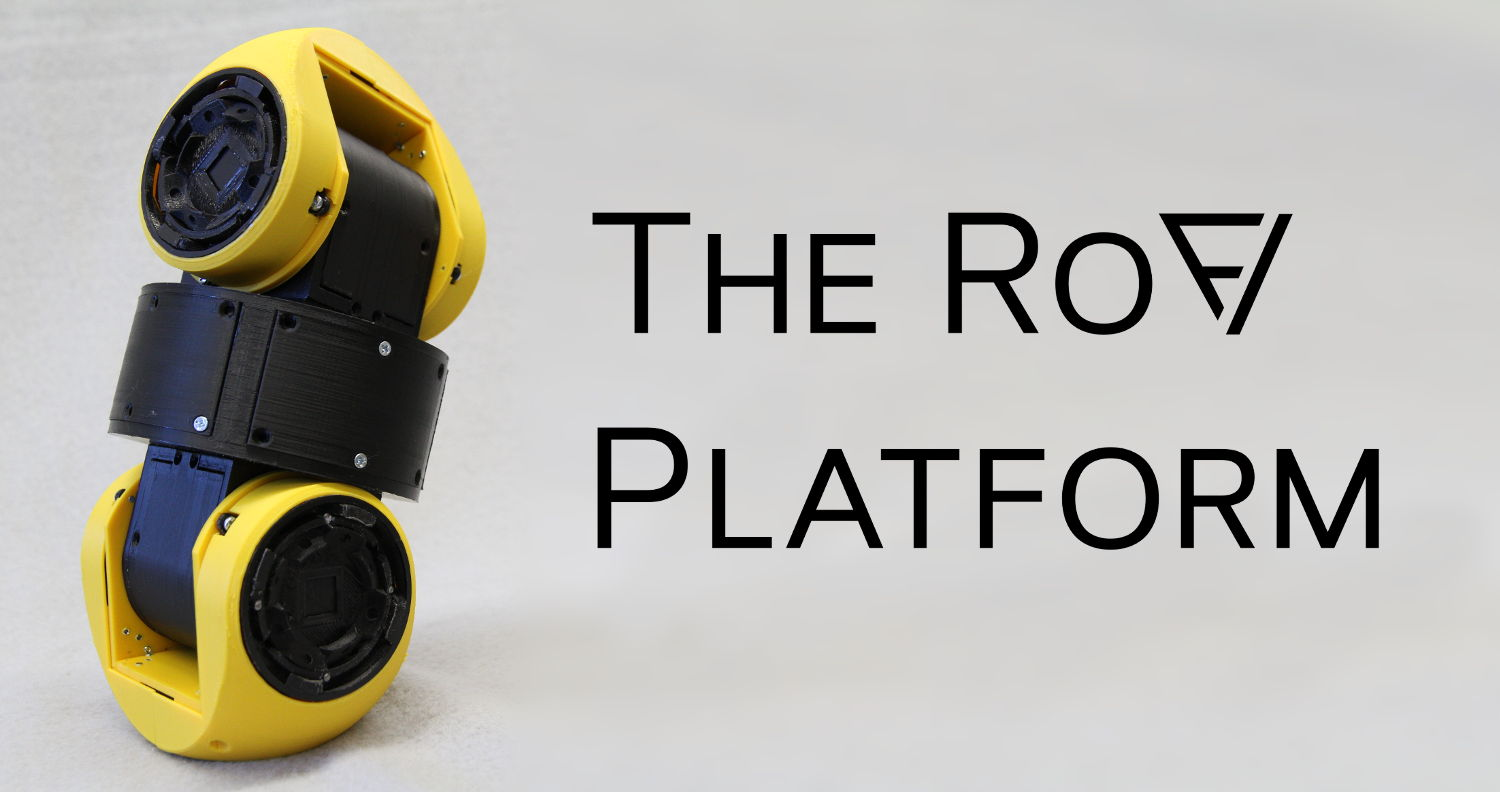
\includegraphics[width=\textwidth,height=\textheight,keepaspectratio]{ assets/rofi-logo.jpg }
    \caption[\acrshort{rofi} logo]{The \acrshort{rofi} platform logo with \gls{universal-module} \cite{rofiweb}}
    \label{fig:rofi-logo}
\end{figure}

% Background --- previous research
The \acrshort{rofi} platform is established in Jan Mrázek's thesis \cite{Mrazek2019thesis}. His thesis focuses on modeling the platform as well as specifying the requirements for modules and even the docking system. In the case of the docking system, his thesis introduces connector-to-connector and connector-to-module communication (\TODO{which both persist to this day}), and the mechanical structure, which was improved over the proposed version.

Even though the thesis (by Jan Mrázek) showcases the connector prototype, that prototype differs a lot from the current version. The more up-to-date version of the connector is described in the paper ``RoFICoM --- First Open-Hardware Connector for Metamorphic Robots'' by Jan Mrázek and Jiří Barnat \cite{MrazekBarnat2019Roficom}.

In the following text (this thesis), the usage of ``prototype'' is used to address the project version before my thesis, and the usage of ``current'' (implementation or version) is to describe the resulting project after the thesis.

% Establishing the problem
\TODO{Even though} the previous work creates the connector, the implementation is in a work-in-progress state. The aim of this thesis is to enhance the firmware of the \acrshort{roficom} to a production-ready state by improving the prototype implementation and adding new features.

% Specifying objectives
The main objectives for this thesis are:
\begin{itemize}
    \item Implement distance measuring into \acrshort{roficom}, which includes implementing an \acrshort{i2c} driver and \TODO{integrating} the \gls{vl53l1x} driver.
    \item Propagate the measurements from the \acrshort{roficom} to the \gls{universal-module}. 
    \item Port the prototype firmware for the \acrshort{roficom} to the production-ready version of the hardware board.
    \item Change motor control in the firmware to use newly added magnetic sensors.
    \item Implement power control --- i.e., reading current and voltage on internal and external powerlines, charging accumulator from internal powerline, and discharging the accumulator to the internal powerline.
\end{itemize}

% Paper structure
The structure of this paper starts with an introduction to the \acrshort{rofi} platform and a description of its components \TODO{in the next chapter}, which is followed by an overview of the prototype firmware implementation and proposes what changes was made to improve it. After that, this thesis focuses on changes made to the \acrshort{roficom} firmware in this thesis. Those changes are distance measuring in the \acrshort{lidar} \autoref{sec:lidar}, \acrlong{bsp} for isolating board-specific code and adapting changes in the board (\autoref{ch:bsp}), and other interesting implementations and their reasoning, followed by the conclusion of this thesis (\autoref{ch:design}). The last chapter (\autoref{ch:rofi-hal}) focuses on changes and updates made to the \acrshort{rofi} \acrlong{hal}.

\chapter[ RoFI ]{ \acrshort{rofi} }
\TODOLIST{
\begin{itemize}
    \item Describe the platform
    \item Universal module
\end{itemize}
}

The \acrshort{rofi} is a platform of distributed self-reconfigurable modular robots developed at the Faculty of Informatics, Masaryk University.

\begin{figure}
    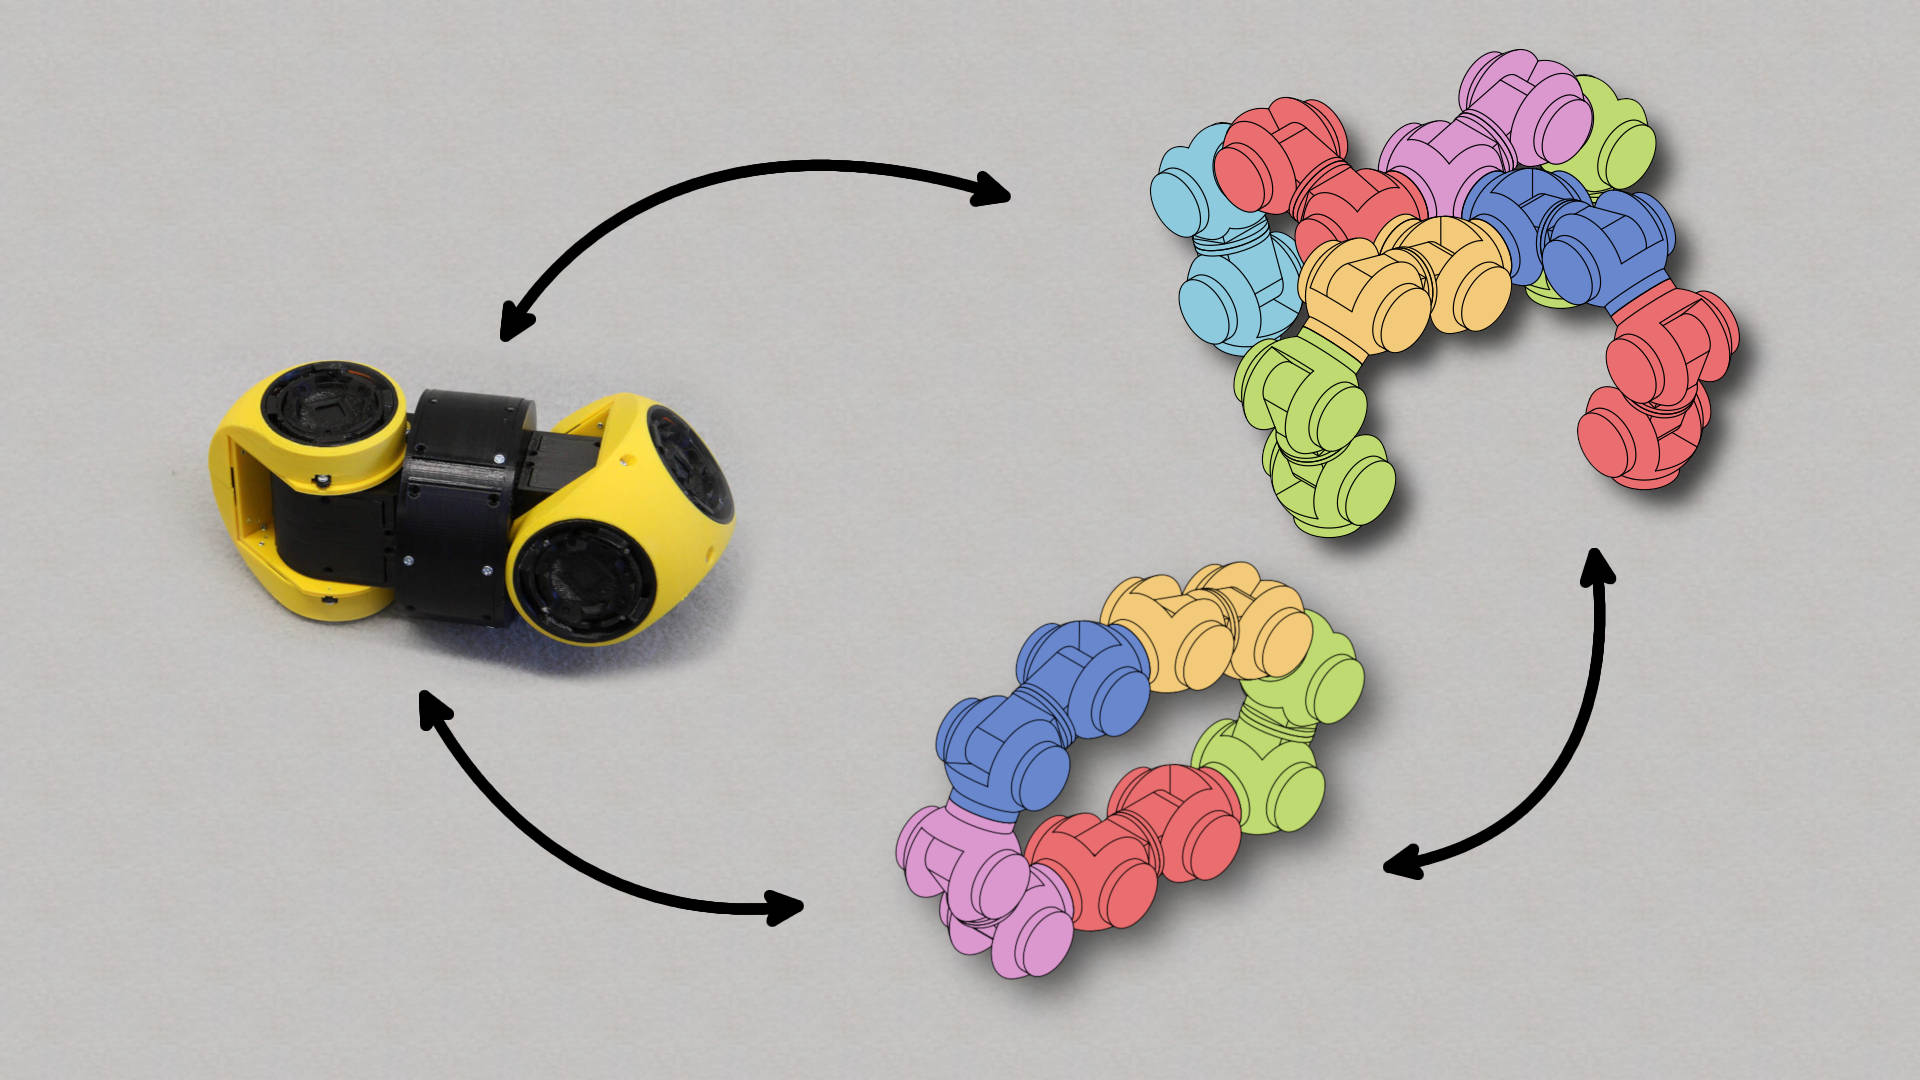
\includegraphics[width=\textwidth,height=\textheight,keepaspectratio]{assets/rofiTransformation.jpg}
    \caption[\acrshort{rofi} transformation]{Illustration of possible \acrshort{rofi} robots transformation from \TODO{\cite{rofiweb}}}
    \label{fig:rofi-transformation}
\end{figure}

The main goal of the \acrshort{rofi} platform is to provide a well-established open-source and open-hardware platform for metamorphic robots. Therefore, source code and hardware schematics are publicly provided in the \TODO{ GitHub repository \footcite[\url{https://github.com/paradise-fi/RoFI}]{rofi-github} }. The primary use case for such a platform is testing reconfiguring algorithms on a hardware platform and further researching this topic rather than \TODO{solving real-world problems}.

The basic building block is the \acrshort{rofi} module, which is an individual module that can connect and communicate with other modules. A \TODO{flock} of connected \acrshort{rofi} modules makes a \emph{\gls{rofibot}}. A specific example of the \acrshort{rofi} module is the \gls{universal-module}.


\section[ Universal Module ]{ \gls{universal-module} }
\TODOLIST{
    \begin{itemize}
        \item ESP32
        \item \acrshort{spi}
        \item \acrshort{uart}
        \item accumulator
        \item EXT and INT power lines
        \item 3 motors
        \item 6 docks
    \end{itemize}
}
\gls{universal-module} \glsdesc{universal-module} The \gls{universal-module} is not designed as an all-in-one module but rather as a module with minimal \TODO{necessary features} that can be used in nearly all systems. Thus, the \gls{universal-module} uses only two sensors: an \emph{inertial measurement unit} (IMU) and a \emph{distance sensor} (\acrshort{lidar}). If other specific sensors are needed, it is expected to use them as their own modules.

An inertial measurement device measures the unit's acceleration, angular velocity and orientation. The measured data can be used in algorithms coordinating the modules.

The distance sensor (\acrshort{lidar}) is placed in the middle of each dock and described in detail in \autoref{sec:lidar}. The \acrshort{lidar} measures the distance from the dock to an obstacle or a surface, which can to help align docks when connecting. The \acrshort{lidar} can scan the environment, which can be useful when the \gls{rofibot} needs to walk upstairs or needs to know about its surroundings.

The module is divided into four components: two bodies and two shoes. The main purpose of shoes is to establish connections with other modules and provide movement. Each shoe contains three docks and \TODO{one joint}. In comparison, the body encloses actuators, electronics, and accumulators. The last \TODO{joint} is situated between the two bodies. In total, the module contains six docks, three \TODO{joints/motors}, and two types of sensors.

\todo{Insert image of \gls{universal-module}}

\subsection{ Architecture }

The docks used in the \gls{universal-module} are called \acrshortpl{roficom}. The \acrshort{roficom} is in detail described and explained in the next \autoref{sec:roficom}.

Each module has a single \emph{control unit} that serves as a centralized control over the actions of the module and all the module's components. Control of the motors is accomplished with a \acrshort{uart} (\acrlong{uart}) \footnote{\url{https://en.wikipedia.org/wiki/Universal_asynchronous_receiver-transmitter}} protocol; whereas in the case of the docks, it is done with \acrshort{spi} (\acrlong{spi}) \footnote{\url{https://en.wikipedia.org/wiki/Serial_Peripheral_Interface}} protocol. Additionally, the control unit manages charging and power connections.

The architecture of the \gls{universal-module} is shown in \autoref{fig:uni-mod-arch}. Each box represents component of the \gls{universal-module} and each line represents connection between components. All connections are done by wires and connections with labels, such as \acrshort{uart}, \acrshort{spi}, represents used protocol or describes the wire (INT, EXT). 

\begin{figure}[ht]
    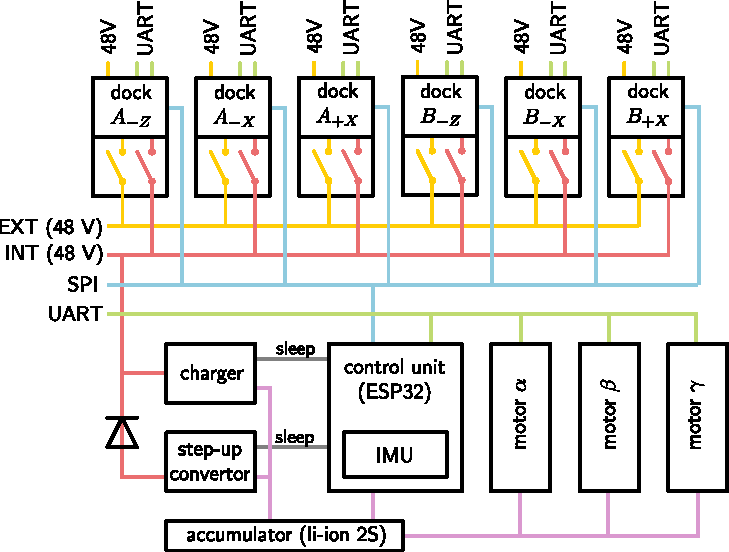
\includegraphics{ assets/universal-module-arch.pdf }
    \caption{The architecture of the \gls{universal-module} from \TODO{\cite[p.~35]{Mrazek2019thesis}}}
    \label{fig:uni-mod-arch}
\end{figure}

\section[ RoFI Communication Mechanism ]{ \acrlong{roficom} } \label{sec:roficom}
\TODOLIST{
\begin{itemize}
    \item Explain \acrshort{roficom}
    \item Describe components --- shirt, clip and body
    \item Describe board --- RAM: 36KB, Flash: 128KB, ...
\end{itemize}
}

\iffalse
<!--
- Connection/Communication part of RoFI Platform
- Designed to be stand-alone unit (so it can be reused in other modules)
- What it consists of?
    - Docks Interaction
    - Docks power-sharing
-->
\fi

\acrlong{roficom}, \acrshort{roficom} for short, is an open-hardware connection system designed for the \acrshort{rofi} platform. \acrshort{roficom} focuses on reusability \TODO{in order to make it easily integrable} into any module for which \acrshort{roficom} provides
communication to other modules. As the name suggests, its primary purpose is to (inter)connect modules. In order to achieve its purpose, the \acrshort{roficom} has a well-defined interface that can be divided into three parts:
\begin{itemize}
    \item mechanical structure,
    \item connector-to-connector interface (communication between two \acrshortpl{roficom}),
    \item connector-to-module interface (communication with the integrated module).
\end{itemize}

\iffalse
\begin{figure}
    % responsive_image path: assets/img/connector/roficom_main_sketch.jpg
    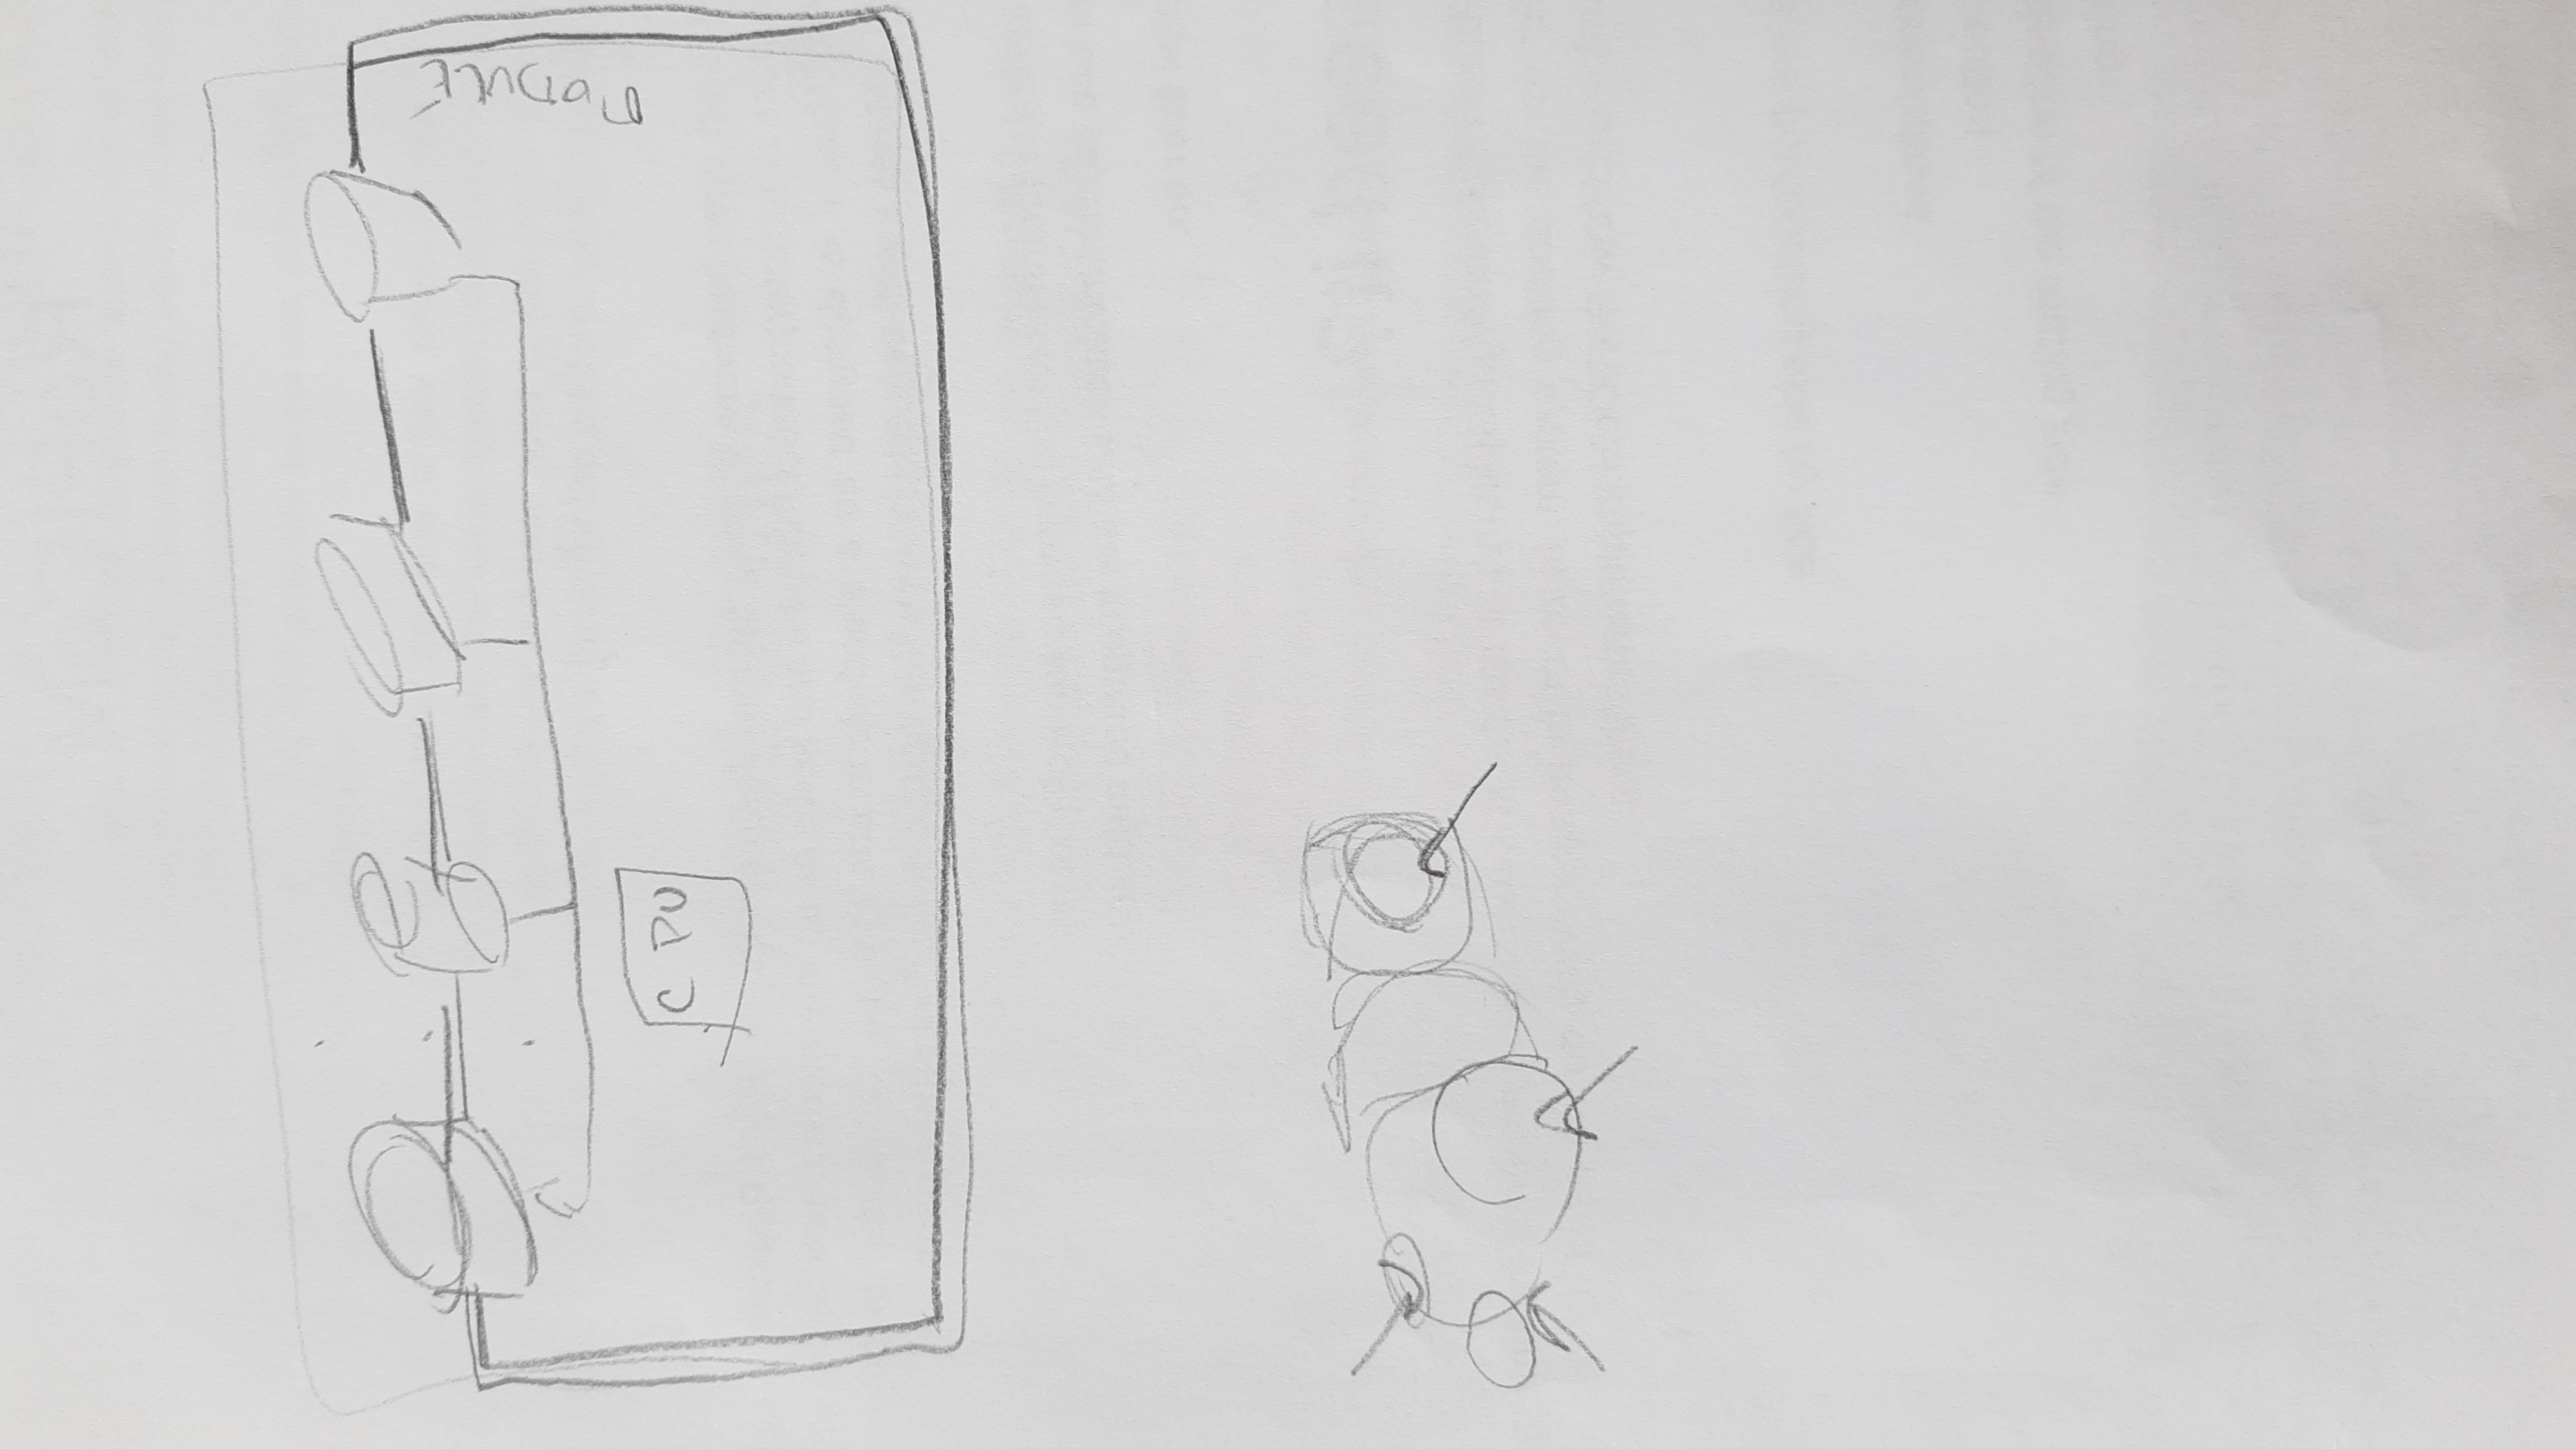
\includegraphics{ roficom_main_sketch.jpg }
    \caption{ \TODO{ The current look of \acrshort{roficom} } }
\end{figure}
\fi

\subsection{Mechanical structure}
\iffalse
<!--
- Describe individual parts: body, clip and skirt
- Magnets in skirt to ease/join the connecting
- extracting and retracting  - motors
- ?? lidar - I2C
-->
\fi

This section describes the mechanical components, their functionality, and the mechanism used to extend and retract the connector. This section summarizes the previously mentioned paper ``RoFICoM'' \cite{MrazekBarnat2019Roficom}, where the structure is explained more deeply.

RoFICoM is built from three main parts: \emph{body}, \emph{clip} and \emph{skirt}. These three parts are shown in \autoref{fig:key-components}

\begin{figure}[ht]
    %responsive_image path: assets/img/connector/dock_key_components.svg 
    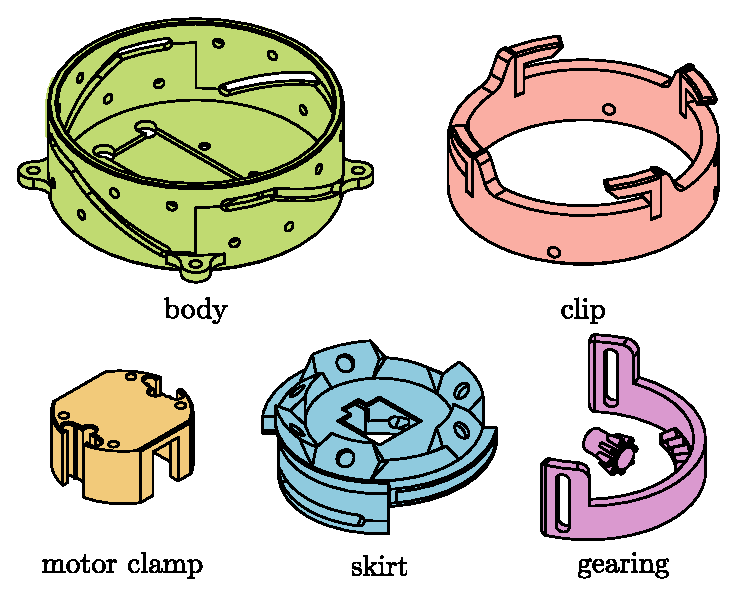
\includegraphics{ dock_components.pdf }
    \caption{ The components of the connector from the paper ``RoFICoM'' \cite{MrazekBarnat2019Roficom} }
    \label{fig:key-components}
\end{figure}

The following text describes the movement of the \acrshort{roficom}'s components in summary to provide an idea of the movement. The detailed description can be found at \cite[p.~10--13]{Mrazek2019thesis}.

The body is a non-movable part that is mounted into the module.
The clip and skirt are essential for establishing strong mechanical connections between two \acrshortpl{roficom}.
The clip component consists of four latches attached to a ring. Those latches get attached while connecting with
other \acrshort{roficom}. While expanding, the clip gets rotated and expanded upward by the motor. In the process, the latches on the mating
side slide under each other, therefore forming a mechanical connection that prevents connectors from being pulled apart.
However, the latches themselves are insufficient for a mechanical connection, as a mutual rotation of the connectors releases
the connection. This is why the skirt is needed, two connected skirts stop the rotation against each other. In order to help ease the process of connection, there are magnets placed in the holes of the skirt. This helps when two connecting sides are slightly misaligned.

The motor that rotates the clip and the skirt is at the body's bottom. The rotation of the clip and the skirt is accomplished by another component, the \TODO{gearing}, which is connected with both the skirt and clip with a \TODO{metal rod?} that spans from the holes in the body up to the skirt. When the motor activates, it rotates the gearing with the two components, and the \TODO{metal rods} move the interconnected components among the hole path in the body, elevating the components.

The \autoref{fig:dock-arrangement} shows the composed components of the \acrshort{roficom}, the color of each component matches from the \autoref{fig:key-components}. The outmost ring part is the body colored green. Next in the body, the pink circle, is the clip. The gearing is the purple half circle connected with the clip by the \TODO{metal rod}.

\begin{figure}
    \centering
    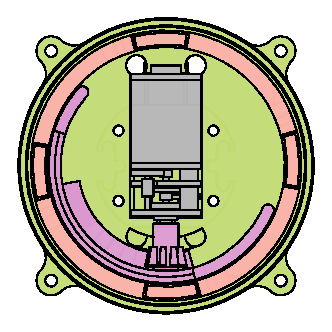
\includegraphics{ assets/dock-arrangement.pdf }
    \caption[Internal arrangement from ''RoFICoM``]{ ''Internal arrangement of the connector --- top view
    without skirt. The motor is shown gray.`` from the paper \cite{MrazekBarnat2019Roficom} }
    \label{fig:dock-arrangement}
\end{figure}

\iffalse
\subsection{ Ratings }
\begin{itemize}
    \item compact, flat layout (diameter 50 mm, thickness 17 mm)
    \item data and power sharing between connected units
    \item load capacity
        \item normal direction: 110 N
        \item shear direction: 50 N
    \item actuation time: less than 0.6 s
    \item genderless, 90-degree symmetrical with automatic orientation detection
\end{itemize}
\fi

\subsection{ Connector to Connector Interface }
\iffalse
<!--
- \acrshort{uart}
- data and power sharing - EXT and INT power lanes 
-->
\fi

A small printed circuit board (PCB) inside the skirt with spring-loaded pins realizes the connector-to-connector connection. This PCB provides both
data and power sharing to the connected module.
\acrshort{roficom} uses \textbf{\acrshort{uart}} transferring frames with specified format and CRC for data communication. Those frames hold ``blobs'' ---
binary data that is transferred between modules. 

\iffalse
\begin{figure}
    % responsive_image path: assets/img/connector/skirt_pins.svg
    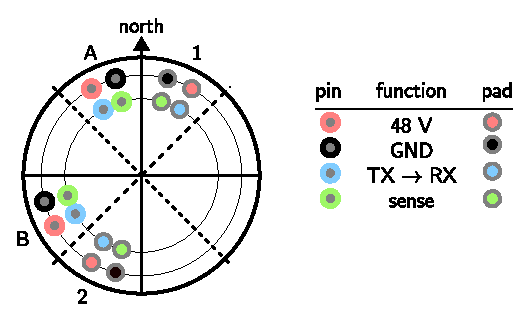
\includegraphics{ skirt_pins.pdf }
    \caption{ \TODO{Graph showing pin layout on PCB inside the skirt} }
\end{figure}
\fi

\subsection{ Connector to Module Interface }
RoFICoM provides an \textbf{\acrshort{spi}} interface for communication between the module and RoFICoM. The communication on the bus is performed
in transactions. Transaction format consists of \textbf{command}, the first 8 bits of a transaction, followed by \textbf{command
data}, then at least 8 bytes pause with connector response. Commands \numrange{0}{127} are reserved for the base connector and are required to be supported by all
connector types. For example, some connector commands are version command, status command, send and receive earlier
mentioned blob.

\iffalse
\subsection{ Motivation of RoFICoM }
<!--
_Requirements_:
- able to connect when docks are not touching side by side
- genderless
- connection in four different orientations
- based on a mechanical connection
- disconnect without the participation of the mating side
- support data and power-sharing
-->

Since the RoFI platform is [grid-based](), it results in several _requirements_
for both the platform and, more importantly for us, the docking system.
In order to answer "Why do we need it?" let's walk through the _requirements_, their cause and how RoFICoM implements them.

<!-- The first _requirement_ is to **allow modules to connect
when they are not touching side by side**, which is caused by the modules being sphere-shaped, resulting in an empty gap between two adjacent modules. RoFICoM solves this by having a [flat design with expanding and retracting](#mechanical-structure) as it connects and disconnects, respectively. -->
RoFICoM has a flat design with ability to expand and retract. This allows RoFICoM to connect over empty space between
adjacent modules. As result modules don't have to be physically touching to be able to connect.

<!-- The _requirement_ of a **genderless** docking system and the **ability to connect in four different orientations** are to limit the
complexity of configuration and reconfiguration. RoFICoM solves this by being 90-degree symmetrical (see figure below). -->
RoFICoM has 90-degree symmetrical design, this is best seen in figure below on the skirt design. Therefore it enables
RoFICoM to connect in **four different orientations** (0°, 90°, 180°, 270°) and makes the connector **genderless**.



RoFICoM forms **strong mechanical connection** using previously mentioned clip and skirt. This feature not only helps RoFICoM stay connected under pressure, but also remain connected without electricity consumption or to avoid limitations of magnetic force.



<!-- It is required to be able to **disconnect without the participation of the mating side** to ease reconfiguration. On top of
that, this allows for connection to passive docks. RoFICoM solves this with its mechanical design of the clip and skirt.
The design enables the connector to expand/retract and thus connect to/disconnect from the mating side independently
of the other side. -->
RoFICoM is designed . This design is accomplished by the clip and skirt, which enables **connection between mating sides** to be established **independently of each other**. Additionally this enables the RoFICoM to connect to passive docks.

Last but not least, the docking system must **support data and power
sharing**, which is used to coordinate and charge modules. RoFICoM solves this with a [connector-to-connector
interface](#connector-to-connector-interface).
\fi


\subsection{ Hardware details } \label{sec:roficom-hw}
\TODOLIST{
\begin{itemize}
    \item MCU
    \item motor
    \item \acrshort{uart}
    \item \acrshort{spi}
    \item \acrshort{i2c}
    \item EXT and INT power lines
\end{itemize}
}

\acrshort{roficom} is actually split into two boards: \TODO{skirt connector} and \TODO{??system board??}, which are connected with a cable connecting the pins between them. The skirt connector board holds \acrshort{lidar} and pins for connector-to-connector connection, where the pins are

\begin{itemize}
    \item \acrshort{uart} pins (TX --- transmit pis and RX --- receive pin),
    \item EXT and INT powerlines,
    \item ``sense`` pins for detecting the orientation of the connection.
\end{itemize}

The internal (INT) powerline can be used to charge the current module or  to charge connected modules from the current one. On the other hand, the external powerline is used only to connect the powerlines of other modules. There are four used pins for the \acrshort{lidar}: two pins for \acrshort{i2c} (SDA and SCL explained in \autoref{sec:i2c}), the \acrshort{lidar}'s enable pin and the \acrshort{lidar}'s interrupt pin. The skirt connector is placed in the middle of the skirt, thus, moving together with the skirt.

The \TODO{system board} contains all other necessary circuits for \acrshort{roficom} to function. It consists of the board's microcontroller, motor, power connections, power management, reading current and voltage from power lines, and \acrshort{spi} interface needed for the connector to module interface. That being said, the circuit for reading the current is not attached at the moment.

% \TODO{ Missing pins and a change in the motor's limit led to the change of MCU }

The magnetic sensors for the motor's retraction and expansion limit could not detect and stop the movement of the motor fast enough, which damaged the \acrshort{roficom}'s case.
As for the magnetic sensors, instead of two pieces, they got increased to an array of ten pieces along the motor's movement path to determine the motor's speed and position more precisely.

The \acrshort{roficom} has microcontroller STM32G071CBUx from the STMicroelectronics. This microcontroller from the STM32G0 family is a high-performance ARM Cortex-M0+ processor. The main features of this microcontroller are:

\begin{itemize}
    \item A maximum clock frequency of \qty{64}{\mega\hertz},
    \item The biggest size of flash memory currently in embedded microcontrollers of \qty{128}{\kilo\byte},
    \item Static RAM of size \qty{36}{\kilo\byte},
    \item 48 available pins.
\end{itemize}

The microcontroller has other functionality, such as CRC calculation, \acrshort{spi}, \acrshort{uart}, \acrshort{i2c}.


\chapter[ RoFICoM --- prototype version and current implementation ]{ \acrshort{roficom} --- prototype version and current implementation }
\TODOLIST{
\begin{itemize}
    \item Project structure/architecture
    \begin{itemize}
        \item suites
        \item Protocol
    \end{itemize}
    \item \texttt{control\_board}
    \item \texttt{stm32cxx}
    \item \texttt{rofi-hal}
\end{itemize}
}

This chapter focuses on the software of the \acrshort{rofi} platform and describes both the state of the software in the prototype implementation and the changes in the current implementation.

% \section{ Project Structure / Architecture}
The \acrshort{rofi} repository is an enormous monolithic (mostly) \verb|C++| project and contains many \acrshort{rofi} related sub-projects. For this thesis, only several sub-projects are essential. Those sub-projects are the \acrshort{roficom}'s firmware, stm32 drivers and \acrshort{rofi} HAL.

% \TODO{Need more introduction or depth description of the structure ??}

\section[ RoFICoM's Firmware ]{ \acrshort{roficom}'s Firmware } \label{sec:roficom-firmware}
\acrshort{roficom}'s firmware is located in the repository at the path \path{RoFI/hardwareModules/RoFICoM/software/control_board/}.

The prototype version had several needed features implemented. Those features were the \lstinline|spiInterface| (the connector to module interface), \lstinline|connInterface| (the connector to connector interface) and motor control. However, since the motor control could not stop the motor fast enough and the magnetic sensors for detecting the motor position changed, \TODO{the motor control firmware needed an update too}. However, the \lstinline|connInterface| is not fully implemented in the prototype and is missing sending all the information defined by the protocol. Due to the addition of lidar, the protocol had to be extended.

\subsection{ Connector-to-Module Protocol }

The protocol for communication hat to be revised because of the addition of distance Measurement to the \acrshort{roficom} and the need to transfer the distance to control unit. After the revision, it was decided that only the status command would be extended by needed information (distance status, measured distance and distance mode).

As previously mentioned the protocol was established in thesis \cite[p.~19--22]{Mrazek2019thesis}, and the following text only describes the final look the status command (not the other commands).

The status command (command of value $1$) is used to request and change the status of the connector, such as expanding or retracting the connector. The module's control unit initiates the communication by sending the command data and waiting for the response.

The format of command data is shown in the \autoref{fig:status-command}, where the upper left corner is the send's data first bit (bit $0$). Each row represents two bytes sent in the transaction, and the rows are sent from top to bottom. The numbers above the format specifies the of the row in that column.

The first row of the command data represents the request state, whereas the second row is a bit mask for the previous row. The mask is used to signal which values of the first row to apply. The meaning of the status bits has the following meaning:

\begin{itemize}
    \item P (position) --- $0$ = retracted connector, $1$ = extended connector,
    \item I (internal powerline) --- $0$ = internal powerline is disconnected, $1$ = internal powerline is connected,
    \item E (external powerline) --- $0$ = external powerline is disconnected, $1$ = external powerline is connected,
    \item DM (distance mode) --- $0$ = autonomous distance mode, $1$ = short distance mode, $2$ = long distance mode. 
\end{itemize}

\begin{figure}
    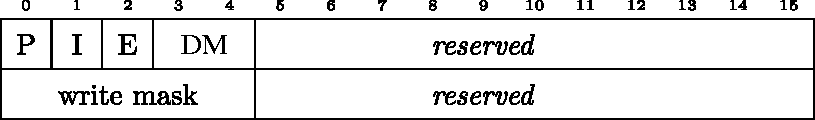
\includegraphics[width=\textwidth,height=\textheight,keepaspectratio]{assets/status_command_new.pdf}
    \caption[Status command data]{The new format of the status command data}
    \label{fig:status-command}
\end{figure}

The prototype version of the protocol already contained the bits P, I and E. The current version added the 2-bits for setting the distance mode. The autonomous distance mode makes the \acrshort{roficom} handle the distance mode of the \acrshort{lidar} and is explained in the \autoref{sec:lidar-autonomous}. The manual handling of the distance mode is done \TODO{via} setting either the short or the long mode, which are described in the \autoref{sec:distance-modes}.

The \autoref{fig:status-response} shows the format of the status command response.

\begin{figure}
    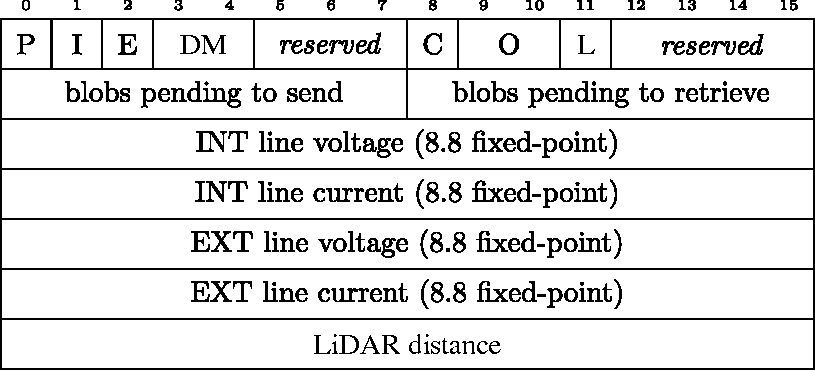
\includegraphics[width=\textwidth,height=\textheight,keepaspectratio]{assets/status_response_new.pdf}
    \caption[Status command response]{The new format of the status command response}
    \label{fig:status-response}
\end{figure}

\begin{itemize}
    \item C (connected) --- $0$ = not connected to mating side, $1$ = connected to the mating side,
    \item O (orientation) --- $0$ = north, $1$ = east, $3$ = south, $4$ = west
    \item L (\acrshort{lidar} status) --- $0$ = error, $1$ = not measured, $2$ = out of range, $3$ = fully valid.
\end{itemize}

Compared to the prototype version of the protocol, the new version added the L bit for the \acrshort{lidar} status and two bytes for the measured distance in millimeters.

\section{ Stm32 Drivers }
\TODOLIST{
\begin{itemize}
    \item already implemented
    \item port files --- portability
    \item to implement --- \acrshort{i2c}
\end{itemize}
}

The \lstinline|stm32cxx| sub-project abstracts and wraps around the bare 
\verb|C| stm32 drivers into nicer \verb|C++| \TODO{classes}. This abstraction allows using the drivers without explicitly handling family-specific code and provides easier and prettier usage rather than using the \verb|C| drivers.

The port files of the \lstinline|stm32cxx| handle the portability or the MCU family-specific code. Folders for family-specific \TODO{abstraction} are under the path \path{RoFI/softwareComponents/stm32cxx/port/}. The \verb|port| files are in the format \verb|{driver}.port.hpp|. For example, the port file for \acrshort{i2c} for the microcontroller of \acrshort{roficom} is in \path{.../stm32cxx/stm32g0xx/i2c.port.hpp}.

Port files follow the same guidelines that the specific code under \lstinline|namespace detail| and it is implemented via \emph{mixins}. However, since \verb|C++| does not natively support mixins, this is done using the \verb|C++| technique called CRTP. CRTP \footnote{\url{https://en.wikipedia.org/wiki/Curiously_recurring_template_pattern}} (Curiously recurring template pattern) is a templated class, which takes the class we wish to extend with our mixin as a template parameter, and implements the mixin functionality on the template class. Such functionality might be enabling a clock for the periphery or \TODO{setting an alternative function on periphery pins}.


The prototype version had \TODO{many drivers (that were needed) implemented}, such as drivers for GPIO, \acrshort{uart}, \acrshort{spi} and more. The current implementation mainly added the driver for \acrshort{i2c} and some smaller additions, namely timer counter, blocking wait for time, and missing family-specific definitions.

\section[ RoFI HAL ]{ \acrshort{rofi} HAL } \label{sec:rofi-hal-desc}
\TODOLIST{
\begin{itemize}
    \item ROFI HAL interface --- prototype vs changes
    \item ROFI HAL implementation esp32    
\end{itemize}
}

\acrlong{hal}, or \acrshort{hal} for short, is part of the \acrshort{rofi} platform that provides an abstraction over the running platform, which can be real hardware or a simulator. It can also be used as an abstraction over different \acrshort{rofi} hardware --- modules with motors, sensors and more --- without changing the user firmware. Therefore, \acrshort{rofi} \acrshort{hal} aims to define a solid and compact interface to make both --- the implementation and the usage simpler.

The \acrshort{rofi} \acrshort{hal} is divided into \emph{interface} and \emph{implementation}. Every change that breaks the previous interface version is costly because that change needs to be reflected in every implementation, which can be a lot. For example, there can be an implementation for each module with specific sensor, motor and multiple simulators. However, due to the addition of \acrshort{lidar}, \TODO{the interface needs an update to reflect this addition}.

The prototype had implementations for the esp32 and simulator. The esp32 is the implementation for the \gls{universal-module}.

The actual changes to the prototype implementation are described later in the \autoref{ch:rofi-hal}.

\chapter[ Distance Measurement --- LiDAR ]{ Distance Measurement --- \acrshort{lidar} } \label{sec:lidar}
\TODOLIST{
\begin{itemize}
    \item \TODO{Walk through \acrshort{lidar} features}
    \item \TODO{Communicating by \acrshort{i2c}}
    \item \TODO{\acrshort{lidar} protocol}
\end{itemize}
}
This chapter describes \acrshort{lidar} and its capabilities, how to use the \gls{vl53l1x} \acrshort{lidar}, which includes communicating with the \gls{vl53l1x} over the bus and using the \gls{vl53l1x} driver provided by the manufacturer. The last section describes the current implementation of the \acrshort{lidar} driver, a \verb|C++| class abstracting the usage of the \gls{vl53l1x} driver.  

\acrshort{lidar}, which stands for \acrlong{lidar}, is a device that measures range. \acrshort{lidar} uses laser and time, in which the light travels to an object or a surface and bounces back to determine the distance. Thus, the results of this technique are very dependent on the ambient light in the measured environment. As such, the \acrshort{lidar} is used for measuring the distance from an object and \emph{3-D scanning}. 3-D scanning is collecting data about the real-world environment into a digital representation. Many industries use \acrshort{lidar} --- one of the most known use cases might be in NASA's Mars helicopter Ingenuity \cite{garmin-lidar}.

\acrshort{roficom} uses \gls{vl53l1x} \acrshort{lidar} from STMicroelectronics. This specific \acrshort{lidar} has the following main features: (All features and description can be found in the part's datasheet \cite{vl53l1x}.)

\begin{itemize}
    \item the ability to accurately measure the range between \qty{4}{\centi\metre} and \qty{4}{\metre},
    \item up to \qty{50}{\hertz} ranging frequency,
    \item single \qty{2.8}{\volt} power supply,
    \item \acrshort{i2c} communication interface with up to \qty{400}{\kilo\hertz} speed,
    \item shutdown and interrupt pins. (However, these pins are not necessary.)
\end{itemize}

Even though \gls{vl53l1x} accurately measures the range between \qty{4}{\centi\metre} and \qty{4}{\metre}, it also measures distances below and above this range, although the measured distance does not have to be accurate. The lidar library, which \acrshort{roficom} uses, deals with inaccuracy by reporting the status of measured data, which is explained later.

The shutdown pin is used to reset the \gls{vl53l1x} by software. That being said, on the actual hardware, the pin is inverted, which results in behavior more similar to enable pin, i.e., the device is enabled when the bus with a shutdown pin is driven high, and the device shuts down when the bus is driven low. This pin does not have to be controlled by software. However, in that case, it still has to be connected to the power supply through a pull-up connector.

On the other hand, the interrupt pin does not require to be connected. This pin signals that the new distance was measured, it is only an output pin. Thus, this pin cannot be used from the controller, and the controller must signal the successful data transfer through \acrshort{i2c}.

The alternative to the interrupt signal is polling. Polling means that the firmware asks the \gls{vl53l1x} periodically whether the measurement data are ready to be transmitted. However, if the period is too long, it is possible to miss some measured data. For example, if the inter-measurement timing (the time between two measurements) was \qty{100}{\milli\second} and the firmware's asking period was \qty{500}{\milli\second}, the firmware could miss four measurements from the \gls{vl53l1x}.

In both cases, the controller should signal the successful read as soon as possible, otherwise the \gls{vl53l1x} would be waiting for the data read,  unable to change the measured data, thus, missing newly measured data.

\section{ Communication }
This section describes details of communication with the \gls{vl53l1x} --- i.e., the protocol used for communication and how the protocol works, usage of the protocol in \gls{vl53l1x}, and the current \acrshort{i2c} implementation for the \gls{vl53l1x} driver. 

\gls{vl53l1x} uses the \acrshort{i2c} communication protocol. The next subsection describes this protocol, if you are familiar with the protocol, you can continue to \autoref{sec:lidar-i2c}.

\subsection[ Inter-Integrated Circuit Protocol ]{ \acrlong{i2c} Protocol } \label{sec:i2c}
\acrshort{i2c}, which stands for \acrlong{i2c}, is a protocol designed for communication between a controller (or more controllers) and multiple peripheral devices. The protocol requires only two lines: SDA (serial data) and SCL (serial clock). Both lines are open-drain with pull-up resistors, which means that the bus driver can drive the bus line low but cannot drive it high. This constraint prevents the collision driving the line both high and low, which would damage the drivers.

The protocol's communication is done in 8-bit packets. The transaction starts with the start condition. After that, every packet is confirmed from the receiving side with one acknowledgment bit, and the transaction ends with the stop condition. Since more peripheral devices can be connected to the \acrshort{i2c} bus, the controller must first address the peripheral to communicate.

The address of a peripheral is a 7-bit (in rare cases 10-bit number). The reason why the address is only 7-bit and not the full 8-bits of the packet is because the last bit indicates the transaction type. The transaction type is either read transaction (the bit is set to 0) or write transaction (the bit is set to 1). The read/write bit is the least significant bit of the packet, and the address is contained in the seven highest bits of the packet (i.e., the address is shifted left by one bit). After the address is sent and met with acknowledgment from the peripheral, the data begins to be transmitted. \TODO{The protocol allows for any length of the data to be transmitted.}

The start condition is when the controller drives the SDA line low before the SCL goes down. The stop condition is when the controller releases SDA (the line goes from low to high) \textbf{after} the SCL line changes to high. It is suggested not to change the SDA line while SCL is high to avoid signaling false stop conditions during data transmission. Note that the acknowledgment bit is negated, i.e., logical 0 on the bus line signals that the peripheral received the packet successfully, whereas logical 1 signals the opposite.


\subsection[ Addressing LiDAR's Registers ]{ Addressing \TODO{\acrshort{lidar}}'s Registers } \label{sec:lidar-i2c} 
\gls{vl53l1x} not only uses an \acrshort{i2c} address but also requires the address of its register, which is a 16-bit number. However, the \acrshort{i2c} protocol only addresses the device, in order to address the device's register, a normal transaction is started, where the first two data packets are the two bytes of the register address. The most significant byte of this index (register address) is sent first, followed by the least significant byte. Sending the index applies to both types of transactions (read and write). That means that to read data from the \gls{vl53l1x}, the controller needs to make two transactions: a write transaction with register index, and the actual read. However, writing data to the \gls{vl53l1x} makes only one write transaction because the index and data \textbf{must} be written together in one transaction.

% \subsection[ I2C Implementation ]{ \acrshort{i2c} Implementation } \label{sec:lidar-i2c-impl}
% \TODOLIST{
% \begin{itemize}
%     \item i2c driver
%     \item \gls{vl53l1x} platform files
% \end{itemize}
% }


\section[ Controlling the VL53L1X ]{ \TODO{ Controlling the \gls{vl53l1x} (Protocol / API)} }
Even though \gls{vl53l1x} has clearly defined read and write operations, there is no public specification of how to control the \gls{vl53l1x}, i.e., how to initialize the \gls{vl53l1x}, start measuring and request the measured data. STMicroelectronics provides and recommends using their software API, in the form of a software driver, to control the \gls{vl53l1x}. The driver is a bare \verb|C| library (not a \verb|C++| library) and is dual licensed under STMicroelectronics' proprietary license and under BSD 3-clause license, which is compatible with \acrshort{rofi}'s MIT license.

STMicroelectronics provides three driver versions: Full API (standard), \acrlong{uld} (\acrshort{uld}) and Ultra Low Power (ULP). The full API, or standard, driver implements a plethora of functionality together with errors and error messages. The \acrlong{uld} strips down the API only to necessary functionality; however, it contains calibration, which can be removed if the space is needed. The Ultra Low Power driver aims for the lowest power usage possible.

The \acrlong{uld} was selected for the \acrshort{roficom} because the full API was too large for the firmware. The prototype firmware already used a lot of the flash memory, around $80\%$ in debug build and above $60\%$ in release build, making the usage of the full API driver unfeasible. The size of the full API driver's release build took up to \qty{19}{\kilo\byte} of the MCU's Flash. In comparison, the release build of \acrlong{uld} takes only \qty{1}{\kilo\byte}. 

The use of \acrshort{uld} resulted in missing errors and error messages previously used with the full API driver. The \acrshort{uld} only reports failures either caused by lidar (signified as value $1$) or from the under-laying layer (\acrshort{i2c} communication). Nevertheless, in both cases, we lose the error message. The precise design of the error handling of the \acrshort{i2c} class (\autoref{sec:i2c}) together with the examination of the error handling of the \acrshort{uld} (\autoref{sec:uld-err}) resulted in some preservation of error information.

\section[ API of the Ultra Lite Driver ]{ API of the \acrlong{uld} } \label{sec:lidar-api}
Because the \acrshort{uld} API is platform independent, it requires the user to implement \acrshort{i2c} communication for the platform (the implementation of \acrshort{i2c} in \acrshort{roficom} is described in \autoref{sec:lidar-i2c-impl}). The UM2510 \cite{um2510} manual explains how to use the \acrshort{uld} API and will be described in this section.

The flow of communication is following:
\begin{enumerate}
    \item Wait for a successful boot of the \gls{vl53l1x}.
    
    \item Initialize the \gls{vl53l1x}.
    
    \item  Set optional settings for the \gls{vl53l1x}, such as changing the \gls{vl53l1x}'s \acrshort{i2c} address, changing the distance mode, changing timings for measurements.
    
    \item Start ranging, i.e., start measuring the data.
    
    \item Wait for the data to be ready --- either by polling or by interrupt.
    
    \item Receive the data from \gls{vl53l1x}.
    
    \item Prepare for the next ranging --- clear the interrupt flag.
    
    \item Either repeat from $5.$ step or stop the measuring.
\end{enumerate}

\todo{Insert API flow diagram}

\subsection{ Error Handling } \label{sec:uld-err}

Since the \acrshort{uld} is a \verb|C| library, the error is signaled by the returned value from every API function. When results other than errors are needed, thy are provided as an ``out'' argument, i.e., a pointer to the given variable.

The error type (\lstinline[breaklines=false]|typedef int8_t VL53L1X_ERROR;|) for the \acrshort{uld} is an 8-bit signed integer. The full API driver defines error values among the definition of the error type; however, this is not the case for the \acrshort{uld}. Even though the \acrshort{uld} does not specify error codes, the code for no error is defined to be $0$. Although the \acrshort{uld} usually returns errors from the underlying \acrshort{i2c} communication, in some cases, the \acrshort{uld} sets the error to value $1$. Thus, the typical error handling of the \acrshort{uld} API calls looks like the code in \autoref{lst:c-error}.

\begin{lstlisting}[
    float=t,
    emph={status != 0}, emphstyle=\underbar,
    caption={Structure of error handling of the \acrshort{uld} function calls.},
    captionpos=b,
    label={lst:c-error}
    ]
VL53L1X_ERROR status;
status = VL53L1X_SensorInit( ... );
if (status != 0) {
    ... // Report error
    return status;
}

status = VL53L1X_StartRanging( ... );
if (status != 0) {
    ... // Report error again
    return status;
}
\end{lstlisting}

\subsection{ Distance Modes } \label{sec:distance-modes}

\gls{vl53l1x} has three distance modes: \emph{short}, \emph{medium} and \emph{long}. Since the \acrshort{lidar} depends on ambient light, this is when distance modes make a difference. Even though short mode can measure only up to \qty{136}{\centi\metre}, it is not as impacted by the ambient light as other modes. The datasheet \cite{vl53l1x} mentions that the short distance mode can measure \qty{135}{\centi\metre} under strong ambient light, which is nearly the same as without ambient light. On the contrary, the ambient light impacts the medium and long modes. Whereas the long mode can measure up to \qty{360}{\centi\metre}, in the strong ambient light, it only measured \qty{73}{\centi\metre}.

The \acrshort{uld} provides only two distance modes: short and long. The representation for modes is \lstinline|1| for the short mode and \lstinline|2| for the long mode. The \acrshort{uld} provides functions \lstinline|VL53L1X_SetDistanceMode()| and \lstinline|VL53L1X_GetDistanceMode()| to set and retrieve the current \gls{vl53l1x} distance mode.

% \subsection{ Timings }

% \todo{ Insert timings diagram }

\subsection{ Timing Budget } \label{TB}

The \emph{timing budget} is the time that \acrshort{lidar} measures the distance. \TODO{ The longer the timing budget, the longer the maximum distance \acrshort{lidar} can measure }, but it comes at the cost of increased power consumption. The user can set the timing budget, which ranges from \qtyrange{20}{1000}{\milli\second}. There are a few constraints on the timing budget. The minimal budget timing that can be used for all distance modes is \qty{33}{\milli\second}; however, the short distance can use lower timings. In order to be able to measure \qty{4}{\metre} in the long distance mode, the timing budget must be at least \qty{140}{\milli\second}.

For the \acrshort{uld}, there is a difference in allowed values \TODO{compared} to the timing budget in the datasheet \cite{vl53l1x}. The allowed values for timing budget in the \acrshort{uld} are only $[15, 20,
33, 50, 100, 200, \qty{500}{\milli\second}]$. \TODO{However, the \qty{15}{\milli\second} timing can only be used for the short distance mode}. The default value is set to \qty{100}{\milli\second}.

\subsection{ Inter-Measurement Period }
The \emph{inter-measurement} period is the time between the consecutive measurements. Therefore the inter-measurement period must be longer than the timing budget. The inter-measurement period is also programmable by the user.

The inter-measurement period must be longer than the timing budget. However, the \acrshort{uld} does not validate this and is left to the user to ensure. Otherwise, the actual inter-measurement period would be double the expected value. The default value is set to \qty{100}{\milli\second}.

\subsection{ Result Data } \label{sec:lidar-result}

The main reason for having \acrshort{lidar} is to be able to measure the distance from the \acrshort{roficom}; thus, receiving the measurements and their correctness is the main \TODO{focus}. The result can be received in two ways, either by requesting the specific result values, such as distance or by receiving all the values at once. The current implementation only uses measured \emph{distance} and the \emph{status} of the measurement.

The distance is measured in millimeters and is saved as two bytes long unsigned number.

\iffalse
\TODO{
\begin{lstlisting}
typedef struct {
    uint8_t Status;
    uint16_t Distance;
    uint16_t Ambient;
    uint16_t SigPerSPAD;
    uint16_t NumSPADs;
} VL53L1X_Result_t;
\end{lstlisting}
}
\fi

\paragraph{\TODO{Status}}

On the contrary, the status is only one byte long but has more a \TODO{complex meaning}. The \acrshort{uld} manual \cite{um2510} documents only five statuses, even though the \gls{vl53l1x} datasheet \cite{vl53l1x} specifies eight. The five statuses with their corresponding values are:
\begin{itemize}
    \item Valid (0)
    \item Sigma failure (1)
    \item Signal failure (2)
    \item Out of bounds (4)
    \item Wraparound (7)
\end{itemize}

The range status of $0$ indicates successful measurement with the measurement data being ready to use.

The sigma failure with value $1$ means that the standard deviation of the measurements had surpassed the expected (normal) values, thus resulting in an error. This error can be fixed by increasing the timing budget.

The signal failure with value $2$ is caused by \gls{vl53l1x} measuring a weak signal. The signal rate is represented as the amplitude of the reflected signal from the target. This failure can happen when the target is too far or is not reflective enough, or there is no target. Since increasing the timing budget increases the maximum measurable distance, it can eliminate this status but does not have to.

The out-of-bounds with value $4$ usually occur when the target is at the maximum possible measurable distance (and is very bright target). Subsequently, the measured results may be inconsistent.

The ``wraparound'' range status of value $7$ is reported when the target is very reflective, and the distance is longer than the limited physical distance measurable by the \gls{vl53l1x}. This distance is \qty{1.3}{\metre} for the short distance mode and \qty{5}{\metre} for the long mode.

\section[ LiDAR Diver ]{ \TODO{ \acrshort{lidar} Driver Abstraction in \acrshort{roficom} } } \label{sec:lidar-driver}

Because most of the \acrshort{roficom} project uses \verb|C++| abstraction, the same was intended for the \acrshort{lidar}. Moreover, the \acrshort{lidar} was designed as an independent library from the \acrshort{roficom} firmware. \TODO{However, the \acrshort{lidar} library depends on the \texttt{stm32cxx} drivers.} The main goal for this driver is to make pleasant abstraction around the actual \verb|C| driver. Having the \acrshort{lidar} driver abstraction enables to change or update of the underlying driver without more or less changing the \acrshort{roficom}'s firmware. The \acrshort{lidar} driver was designed to keep communication flow similar to the \verb|C| driver (as described in \autoref{sec:lidar-api}).The \acrshort{lidar} is supposed to be \emph{hot-pluggable}, which means it can be inserted or removed at any time without restarting or crashing the system. Since the \acrshort{lidar} itself does not have to be plugged into the \acrshort{roficom}, it was desired to have the management of the \acrshort{lidar} state more explicit. The states are: \acrshort{lidar} is not present, \acrshort{lidar} is present but not yet initialized, \acrshort{lidar} is initialized but not measuring, and last, \acrshort{lidar} is measuring. 

\subsection{Error handling}
Managing state goes in hand with error handling since every operation can fail by either \acrshort{i2c} failing, \verb|C| driver failing, or simply by the fact the \acrshort{lidar} is not plugged in. Before considering the error handling, it is important to mention that the operations of \gls{vl53l1x} differ in the returned value. For example, some function returns the distance mode, the measurement result, or in most cases, they do not return any value; however, all of them can fail.

There are several choices for considering error handling in \verb|C++|. The first choice that comes to mind is exceptions. However, they are not suitable for embedded programming due to the overhead they bring and thus cannot be used. Another solution might be returning the error and passing in other return values as output argument (e.g., pointer or reference). This solution has mainly two issues. The first issue is that every function call needs to be explicitly checked whether it succeeded, significantly cluttering the code. The second issue is that there needs to be a variable in the caller function for each return value. This complicates the code; for example, consider what needs to be done to check whether the measured data are ready to receive from the \gls{vl53l1x}. Firstly, there needs to a \lstinline|bool| variable in the current scope that will hold the readiness of the \gls{vl53l1x}, then the function call to get the readiness; after that, there would be a check whether anything failed, and if not, finally, the check whether the data is ready or not. This produces code that is much more complicated than having a simple check in the form \lstinline[breaklines=false]|if (lidar.getMeasurementDataReady()) {...}|.

\verb|C++23| contains a new mechanism for error handling the \lstinline|std::expected|, similar to Rust's \lstinline|Result| or Haskell's \lstinline|Either|. However, at the time of writing, the project is using \verb|C++20| since not all the features of \verb|C++23| are yet implemented in used compilers. Fortunately, the \acrshort{rofi} project contains implement of the concept under the name \lstinline|Result| under the Atoms project. Atoms are helper libraries for the \acrshort{rofi} project, and the \lstinline|Result| can be found under the path \path{RoFI/softwareComponents/atoms/include/atoms/result.hpp}.

The \lstinline|Result| contains either \emph{value} or \emph{error}. The \lstinline|Result| cannot contain both. It is similar to the \lstinline|std::optional|, although it contains more information about the error. Both the value and error can be any \TODO{type}. The \lstinline|Result| provides the ability to check whether the result contains value or error (with either \lstinline|bool| operator or \lstinline|has_value()| method), receive the underlying value or error, and \emph{monadic functions}. If you are unfamiliar with monadic functions, they allow you to work on the wrapped value (i.e., value or error in the case of \lstinline|Result|) rather than the \lstinline|Result| itself. Those functions save us from the constant checking of whether the result contains value or error. The monadic functions for the \lstinline|Result| are \lstinline|and_then()|, \lstinline|or_else()| and \lstinline|transform()|. The \lstinline|and_then()| method applies its argument (callable function) on the value of the \lstinline|Result| only if the value is present; otherwise, it returns the error. Similarly, the \lstinline|or_else()| returns value if it contains value; otherwise, returns result of its argument (again callable function). The \lstinline|transform()| and \lstinline|transform_error()| are used to transform the type of value or error, respectively.

Even though the return value types differ for many functions, the error type is the same for all the functions \TODO{; thus, it is important choice}. The default error type for the \lstinline|Result| is \verb|C++|'s \lstinline|std::string|. However, \lstinline|std::string| is a very robust and heavy library (in an embedded context), which means it is unsuitable for the firmware. Two alternatives were considered --- \lstinline|std::string_view| and base number (or an enum). The \lstinline|std::string_view| was chosen since it allows error detection when developing. However, all functions are implemented in a way to allow for easy error type change. Every function returns the error wrapped by function \lstinline|errorMessage( error )|. The function \lstinline|errorMessage()| converts the bare error (in this case, the error returned by the \gls{vl53l1x} driver) to the \acrshort{lidar}'s error. Thus, when changing the error type for the \acrshort{lidar}, only the \lstinline|error_type| member and the \lstinline|errorMessage()| function must be changed.

\subsection{ Usage of the driver }

\begin{figure}[ht]
    % generated by Plantuml 1.2023.6       
\definecolor{plantucolor0000}{RGB}{24,24,24}
\definecolor{plantucolor0001}{RGB}{255,255,255}
\definecolor{plantucolor0002}{RGB}{241,241,241}
\definecolor{plantucolor0003}{RGB}{0,0,0}
\begin{tikzpicture}[yscale=-1
,pstyle1/.style={color=plantucolor0000,fill=plantucolor0002,line width=0.5pt}
,pstyle2/.style={color=plantucolor0000,line width=0.5pt}
,pstyle3/.style={color=plantucolor0000,line width=1.0pt}
,pstyle4/.style={color=plantucolor0000,fill=plantucolor0000,line width=1.0pt}
,scale=0.3, every node/.style={scale=0.3}
]
\draw[color=plantucolor0001,fill=plantucolor0000,line width=1.0pt] (16pt,78.5659pt) ellipse (10pt and 10pt);
\draw[pstyle1] (61.5pt,78.5659pt) arc (180:270:25pt) -- (86.5pt,53.5659pt) -- (229.3432pt,53.5659pt) arc (270:360:25pt) -- (254.3432pt,78.5659pt) -- (254.3432pt,78.8315pt) arc (0:90:25pt) -- (229.3432pt,103.8315pt) -- (86.5pt,103.8315pt) arc (90:180:25pt) -- (61.5pt,78.8315pt) -- cycle;
\draw[pstyle2] (61.5pt,79.8628pt) -- (254.3432pt,79.8628pt);
\node at (128.4105pt,58.5659pt)[below right,color=black]{missing};
\node at (66.5pt,84.8628pt)[below right,color=black]{LiDAR is not plugged in};
\draw[pstyle1] (455pt,78.5659pt) arc (180:270:25pt) -- (480pt,53.5659pt) -- (761.8415pt,53.5659pt) arc (270:360:25pt) -- (786.8415pt,78.5659pt) -- (786.8415pt,78.8315pt) arc (0:90:25pt) -- (761.8415pt,103.8315pt) -- (480pt,103.8315pt) arc (90:180:25pt) -- (455pt,78.8315pt) -- cycle;
\draw[pstyle2] (455pt,79.8628pt) -- (786.8415pt,79.8628pt);
\node at (572.6031pt,58.5659pt)[below right,color=black]{uninitialized};
\node at (460pt,84.8628pt)[below right,color=black]{LiDAR is plugged in, but not yet initialized};
\draw[pstyle1] (942pt,78.5659pt) arc (180:270:25pt) -- (967pt,53.5659pt) -- (1233.3431pt,53.5659pt) arc (270:360:25pt) -- (1258.3431pt,78.5659pt) -- (1258.3431pt,78.8315pt) arc (0:90:25pt) -- (1233.3431pt,103.8315pt) -- (967pt,103.8315pt) arc (90:180:25pt) -- (942pt,78.8315pt) -- cycle;
\draw[pstyle2] (942pt,79.8628pt) -- (1258.3431pt,79.8628pt);
\node at (1061.7626pt,58.5659pt)[below right,color=black]{initialized};
\node at (947pt,84.8628pt)[below right,color=black]{LiDAR is intialized and ready to measure};
\draw[pstyle1] (1465.5pt,78.5659pt) arc (180:270:25pt) -- (1490.5pt,53.5659pt) -- (1669.9667pt,53.5659pt) arc (270:360:25pt) -- (1694.9667pt,78.5659pt) -- (1694.9667pt,78.8315pt) arc (0:90:25pt) -- (1669.9667pt,103.8315pt) -- (1490.5pt,103.8315pt) arc (90:180:25pt) -- (1465.5pt,78.8315pt) -- cycle;
\draw[pstyle2] (1465.5pt,79.8628pt) -- (1694.9667pt,79.8628pt);
\node at (1538.86pt,58.5659pt)[below right,color=black]{measuring};
\node at (1470.5pt,84.8628pt)[below right,color=black]{LiDAR is non-stop measuring};
\draw[pstyle3] (26.04pt,78.5659pt) ..controls (35.03pt,78.5659pt) and (48pt,78.5659pt) .. (56.03pt,78.5659pt);
\draw[pstyle4] (61.43pt,78.5659pt) -- (52.43pt,74.5659pt) -- (56.43pt,78.5659pt) -- (52.43pt,82.5659pt) -- (61.43pt,78.5659pt) -- cycle;
\draw[pstyle3] (254.78pt,78.5659pt) ..controls (311.1pt,78.5659pt) and (383.74pt,78.5659pt) .. (449.46pt,78.5659pt);
\draw[pstyle4] (454.58pt,78.5659pt) -- (445.58pt,74.5659pt) -- (449.58pt,78.5659pt) -- (445.58pt,82.5659pt) -- (454.58pt,78.5659pt) -- cycle;
\node at (272.75pt,59.5659pt)[below right,color=black]{LiDAR got plugged in};
\draw[pstyle3] (260.27pt,96.5459pt) ..controls (267.35pt,97.7959pt) and (271.75pt,98.5659pt) .. (271.75pt,98.5659pt) ..controls (271.75pt,98.5659pt) and (437.75pt,98.5659pt) .. (437.75pt,98.5659pt) ..controls (437.75pt,98.5659pt) and (444.33pt,97.8459pt) .. (454.99pt,96.6859pt);
\draw[pstyle4] (254.97pt,95.6159pt) -- (263.1515pt,101.0988pt) -- (259.8961pt,96.4726pt) -- (264.5223pt,93.2171pt) -- (254.97pt,95.6159pt) -- cycle;
\node at (272.75pt,82.5659pt)[below right,color=black]{LiDAR got unplugged};
\draw[pstyle3] (787.19pt,78.5659pt) ..controls (835.55pt,78.5659pt) and (888.32pt,78.5659pt) .. (936.52pt,78.5659pt);
\draw[pstyle4] (941.77pt,78.5659pt) -- (932.77pt,74.5659pt) -- (936.77pt,78.5659pt) -- (932.77pt,82.5659pt) -- (941.77pt,78.5659pt) -- cycle;
\node at (805.5pt,59.5659pt)[below right,color=black]{lidar.Initialize()};
\draw[pstyle3] (1258.17pt,78.5659pt) ..controls (1323.93pt,78.5659pt) and (1398.99pt,78.5659pt) .. (1460.08pt,78.5659pt);
\draw[pstyle4] (1465.2pt,78.5659pt) -- (1456.2pt,74.5659pt) -- (1460.2pt,78.5659pt) -- (1456.2pt,82.5659pt) -- (1465.2pt,78.5659pt) -- cycle;
\node at (1276.25pt,59.5659pt)[below right,color=black]{lidar.StartMeasuring()};
\draw[pstyle3] (1465.41pt,95.6959pt) ..controls (1453.84pt,97.4259pt) and (1446.25pt,98.5659pt) .. (1446.25pt,98.5659pt) ..controls (1446.25pt,98.5659pt) and (1277.25pt,98.5659pt) .. (1277.25pt,98.5659pt) ..controls (1277.25pt,98.5659pt) and (1272.04pt,97.9759pt) .. (1263.42pt,97.0059pt);
\draw[pstyle4] (1258.28pt,96.4259pt) -- (1266.7644pt,101.4275pt) -- (1263.2473pt,96.9969pt) -- (1267.6779pt,93.4798pt) -- (1258.28pt,96.4259pt) -- cycle;
\node at (1278.25pt,82.5659pt)[below right,color=black]{lidar.StopMeasuring()};
\draw[pstyle3] (259.76pt,66.6859pt) ..controls (413.94pt,48.6859pt) and (689pt,16.5659pt) .. (689pt,16.5659pt) ..controls (689pt,16.5659pt) and (855pt,16.5659pt) .. (855pt,16.5659pt) ..controls (855pt,16.5659pt) and (933.06pt,36.3159pt) .. (1001.06pt,53.5259pt);
\draw[pstyle4] (254.78pt,67.2659pt) -- (264.1862pt,70.1854pt) -- (259.7457pt,66.6809pt) -- (263.2502pt,62.2403pt) -- (254.78pt,67.2659pt) -- cycle;
\node at (690pt,7.5659pt)[below right,color=black]{LiDAR got unplugged};
\draw[pstyle3] (259.73pt,55.3759pt) ..controls (336.97pt,37.7659pt) and (430pt,16.5659pt) .. (430pt,16.5659pt) ..controls (430pt,16.5659pt) and (596pt,16.5659pt) .. (596pt,16.5659pt) ..controls (596pt,16.5659pt) and (1276pt,53.5659pt) .. (1276pt,53.5659pt) ..controls (1276pt,53.5659pt) and (1378.98pt,62.0359pt) .. (1465.07pt,69.1159pt);
\draw[pstyle4] (254.66pt,56.5359pt) -- (264.3253pt,58.4284pt) -- (259.5341pt,55.421pt) -- (262.5415pt,50.6298pt) -- (254.66pt,56.5359pt) -- cycle;
\node at (431pt,7.5659pt)[below right,color=black]{LiDAR got unplugged};
\end{tikzpicture}

    \caption[Diagram of \acrshort{lidar}'s state]{\TODO{THIS WILL BE REPLACED lidar state}}
    \label{fig:lidar-state}
\end{figure}

Since the \acrshort{lidar}'s current (only) requirement is always to measure the distance, the firmware accounts for two states --- actively measuring and uninitialized (or unable to measure). The \verb|Measuring| in the figure above stays the same as the actively measuring. However, the state ``unable to measure'' is combined from states \verb|Missing|, \verb|Uninitialized| and \TODO{partially} \verb|Initialized|. These two new states make state handling easier in the code. The state ``unable to measure'' is handled by the function \lstinline|lidarInit()|, and the state \verb|Measuring| is handled by \lstinline|lidarGet()|. The main purpose of \lstinline|lidarInit()| is to initialize correctly the device and start measuring. On the other hand, the function \lstinline|lidarGet()| expects the device to be correctly initialized and measuring. The purpose of \lstinline|lidarGet()| is to check whether the distance is measured, and if it is, save the measurements for the next transfer to the \TODO{module's control unit}.

Those two functions can call each other because if anything fails in the process (in both functions), the device probably needs to be initialized again. On the contrary, when the \lstinline|lidarInit()| succeeds, it is safe to call \lstinline|lidarGet()|. \lstinline|lidarGet()| calls itself to ensure the latest measurements are saved. It is important to note that not receiving the data (i.e., the data is not ready yet) is not a failure and only means it is necessary to check on the data again. Otherwise, the measured value would never be received --- the device would get initialized again before the first measurement.

Nevertheless, the previous implementation would result in infinite indirect recursion; to avoid the recursion, the current implementation uses \lstinline|IdleTask::defer()|. \lstinline|IdleTask| is a class that provides scheduling function calls; the scheduled functions are called with \lstinline[breaklines=false]|IdleTask::run()|. The usage of scheduled function calls allows the firmware to schedule other routines between the two lidar functions, and handle necessary tasks, such as \acrshort{spi} communication.

\subsection{ Autonomous Distance Mode } \label{sec:lidar-autonomous}

The \acrshort{lidar} driver provides one more additional distance mode than is described in \autoref{sec:distance-modes}. This mode is completely handled by \acrshort{lidar} driver and in reality sets the two provided distance modes by the \acrshort{uld}. The autonomous does not change the set timings and instead works with the default ones, which were found suitable for most measurements.

The changes in the underlying mode of the autonomous mode are dependent on the status and distance of successful measurement. The autonomous mode starts in long mode, and if the measurement is valid (signaled by the status value) and the measured is under a specified threshold under its maximum measurable distance, the mode is set to short. If there is invalid measurement while in short mode, such as sigma failure, out of bounds, or wraparound, the distance is set to long mode.


\chapter[ Board Support Package ]{\acrlong{bsp}} \label{ch:bsp}
\TODOLIST{
\begin{itemize}
    \item \acrshort{bsp} = providing i2c functions to \acrshort{lidar} library + easier portability
    \item \acrshort{bsp} = global namespace \lstinline{Gpio::Pin} initialization is **UB**
\end{itemize}
}

Most of the \TODO{development was done} on the prototype board, but it was expected to move to the production-ready (current) version of the hardware board. This was important, especially because the MCU's case changed, which resulted in pin changes and the addition of magnetic sensors for the motor. An easier transition is accomplished by using \acrshort{bsp}.

\acrlong{bsp}, or \acrshort{bsp} for short, is a layer of abstraction specifying  \TODO{minimal needed hardware requirements} for the project and procedures for board initialization. For example, needed pins and peripherals, such as \acrshort{i2c}. 

The main benefit and use case for \acrshort{bsp} is having all board-specific code in one place. The code typically used in \acrshort{bsp} is pin definitions, initialization routines and overall board initialization.

\acrshort{bsp} is usually used in an embedded environment and provides many benefits. Not only it abstracts hardware details, but also it establishes single source of truth for pin definitions, which is less error-prone than having them defined at multiple places. \acrshort{bsp} assures correct initialization of the board at single place. Having everything at a single point enables easier portability across different board versions. The abstraction allows for using the components defined in \acrshort{bsp} in different independent parts of the project. 

In \acrshort{roficom}, \acrshort{bsp} is implemented as two files: \verb|bsp.hpp| and \verb|bsp.cpp|. The \verb|bsp.hpp| header file contains all declarations of pins and peripheral drivers, which live in namespace \lstinline{bsp} and are exposed for use in \acrshort{roficom}. However, the function \lstinline{bsp::setupBoard()} \textbf{must} be called before any pin or driver is accessed. The function \lstinline{bsp::setupBoard()} initialized the board, pins and drivers provided in the \lstinline{bsp} namespace. The header file provides the declaration of function \lstinline{dbgInstance}, which is a function that \acrshort{roficom} uses for debugging with a \TODO{ \texttt{uart} } driver. \verb|bsp.hpp| depends on the external function \lstinline|SystemCoreClockUpdate()|, which is a \TODO{platform-dependent function} that needs to be called after the board clock has been setup. On the contrary, the \verb|bsp.cpp| defines and implements everything declared in \verb|bsp.hpp|. 

\verb|bsp.hpp| acts as an interface specifying what drivers and pins \acrshort{roficom} needs to function; however, since those pins and drivers are stored as global variables in namespace \lstinline{bsp}, the interface should be kept as minimal as possible to save space in the global space. On the other hand, \verb|bsp.cpp| acts as an implementation of this interface and should mainly correctly set up the board, pins, and drivers for usage; that means the \verb|bsp.cpp| can use pins and drivers that are not exposed as it needs to meet the interface specification.

To illustrate the main benefit of the \acrshort{bsp}, imagine a scenario where MCU on the board must be replaced with a different family, thus, changing the pin layout. In this scenario, it would be only to change the \verb|bsp.cpp| file with pin definitions (and if not already present implementation of drivers), but the \verb|bsp.hpp| and components built on top of that would be left unchanged and still work.

\section[ Gpio::Pin Initialization ]{ \lstinline|Gpio::Pin| Initialization }
\lstinline{Gpio::Pin} initialization is the most notable and important change in \lstinline{bsp} that differs from all other uses in \acrshort{roficom}. \acrshort{roficom} uses the expression \lstinline{GpioA[ 9 ]} to specify used pins. \lstinline{GpioA}, \lstinline{GpioB} and \lstinline{GpioC} are global objects provided by the \lstinline{Gpio} driver. At the time of writing, the initialization order of global variables across multiple translation units is not defined by the language specification. As a result, \lstinline{bsp} cannot use \lstinline{GpioA}, ..., for pin definitions and instead uses the \lstinline{Gpio::Pin} structure initialization, where the first argument is the pin position. The second argument is \TODO{the GPIO line defined by STMicroelectronics}.

\chapter{ Implementation --- Design Decisions } \label{ch:design}
This chapter discusses interesting design decisions and explains their reasoning. \TODO{Mention the following sections}.

\section[ I2C driver ]{ \acrshort{i2c} driver }

The \gls{vl53l1x} requires for its communication the \acrshort{i2c} protocol, which is not present in the prototype version of the firmware. This section explains the decisions in designing the implementation for the \lstinline|stm32cxx| \acrshort{i2c} driver. 

The \acrshort{i2c} driver lies with other \verb|stm32| drivers in a project at path \path{RoFI/softwareComponents/stm32cxx/src/drivers/}.

The driver contains class \lstinline|I2C|, \lstinline|SdaPin| and \lstinline|SclPin|, to make the pins distinguishable from \lstinline|Gpio::Pin|, i.e., when constructing the \lstinline|I2C| the following construction, where \lstinline|pinSda| and \lstinline|pinScl| are \lstinline|Gpio::Pin|s, \lstinline|I2C(..., pinSda, pinScl)| would fail to compile. On the other hand, the construction \lstinline|I2C(..., SdaPin( pinSda ), SclPin( pinScl ) )| compiles. It also ensures that swapping the two pin classes would not compile, i.e., \lstinline|I2C(..., SclPin( ... ), SdaPin( ... ) )| would not compile.

The \acrshort{i2c} driver provides two functions \lstinline|read| and \lstinline|write|. Those functions take the \acrshort{i2c} address of the peripheral and data container. There are also \lstinline|unsafe| variants of these functions that are used in \acrshort{lidar} \acrshort{i2c} implementation %\autoref{sec:lidar-i2c-impl}
that take the raw buffer and its size instead of a container. Since the \lstinline|read| and \lstinline|write| are templated functions, they use private functions to implement them. These private functions are not templated and take the raw buffer and size. Using a slim templated function with an inner function that is not templated reduces the size of generated functions from the template but allows the usage of a generalized function.

\subsection{ Error handling }

Since the two functions only take the arguments either for reading from or writing to the given argument, the functions are free to return anything. In this case, they return an error. Because the \acrshort{i2c} driver is used in \acrshort{lidar} \acrshort{i2c}, the error values are chosen to be compatible with error handling in the \acrshort{uld} \autoref{sec:uld-err}. The \acrshort{i2c} error enum has the following errors:
\begin{itemize}
    \item \emph{Valid} value $0$ --- this is to be compatible with the \acrshort{uld} error reporting,
    \item \emph{Reserved} $1$ --- Reserved for the error reported by the \acrshort{uld},
    \item \emph{NotAcknowledge} = 2 --- The acknowledgment bit was not signaled after the 8 bits were transmitted,
    \item \emph{BusError} = 3 --- Bus error signals misplaced start or stop condition,
    \item \emph{ArbitrationLoss} --- Arbitration loss occurs when two masters start transmitting at the same time,
    \item \emph{OverrunUnderrun} --- Overrun is when the newly sent 8-bits are read before the previous 8-bits were read, thus, resulting in data loss. On the other hand, Underrun is when the 8-bits are sent from the data register before the new 8-bits are written into the register, resulting in sending the same 8-bits of data a second time,
    \item \emph{BufferOverflow} --- Buffer overflow happens when the receiving data are longer than the allocated buffer to store those data. The data are read until the end of the buffer and the error is reported.
\end{itemize}

\section{ Motor driver }

As previously mentioned in the \autoref{sec:roficom-hw}, the prototype version of the motor's driver could not stop the motor's rotation fast enough and damaged the \acrshort{roficom}'s case. That resulted in addition of magnetic sensors and the motor driver had to updated. This section explains the current implementation of the driver.

The number of magnetic sensors increased from two to array of ten among the movement path of the gearing. The gearing contains a small magnet that activates the sensors while moving near them. While testing the movement, it was observed that at the same multiple sensors can detect the magnet, which influenced the way the current position is measured.

The current position is measured as a sum of the positions of active pins divided by the count of active pins, further divided by the position of the last pin. The pins are indexed from $\numrange{0}{9}$, where the gearing in the retracted position activates the sensor pin $0$ and the sensor pin $9$ is active in an expanded state. Such indexing should mean that the count of active pins should always be at least one; however, due to the movement or \TODO{malfunction}, the count can be zero, resulting in a division by zero and crashing the whole system. The measured position ranges from $0$ to $100$ (the calculated value times $100$) and sets explicitly the value $-1$ for error in measuring (i.e., zero active sensors). Explicitly setting the error value allows stopping the motor; otherwise, it could run indefinitely, damaging the structure. 

\begin{figure}
    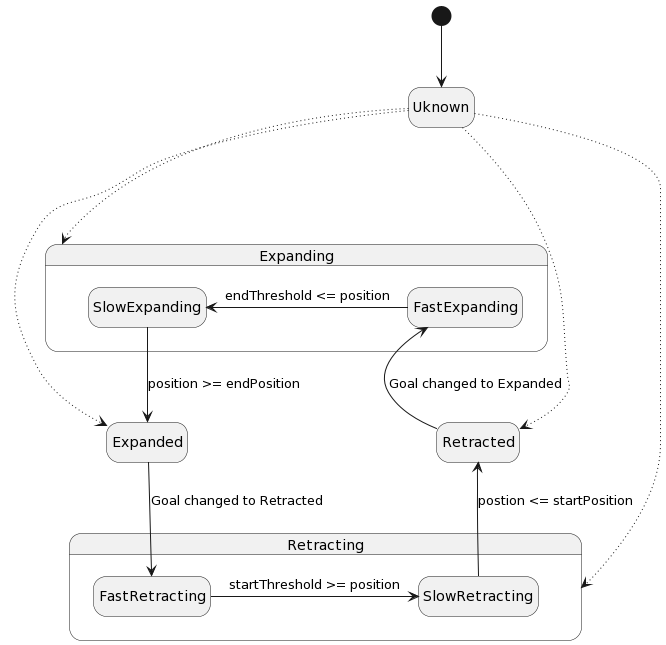
\includegraphics[width=\textwidth,height=\textheight,keepaspectratio]{assets/motor-state-diagram-wip.png}
    \caption{Diagram of motor's state}
    \label{fig:motor-state}
\end{figure}

The \autoref{fig:motor-state} shows the possible states and their transition in the motor driver. The most important states are \lstinline|Retracted| and \lstinline|Expanded| as they indicate the requested position (the motor's goal). The modeled states in the driver are: \lstinline|Retracted|, \lstinline|Expanded|, \lstinline|Retracting|, \lstinline|Expanding| and \lstinline|Unknown|. The \lstinline|Unknown| state indicates the initial state before the position is calculated; this state can change into any other state based on the set goal and current position. The \lstinline|Expanding| is the transition from the \lstinline|Retracted| state to the \lstinline|Expanded| state; similarly, the \lstinline|Retracting| state is the transaction from the \lstinline|Expanded| state to the \lstinline|Retracted| state. Both states (\lstinline|Expanding| and \lstinline|Retracting|) can be split into two more states: Fast and Slow. The Fast state utilizes the whole power of the motor, and upon reaching a specified threshold position, the state changes to the Slow one, which, on the contrary, slows the motor in order to stop the movement before reaching the physical end in the mechanical structure.

The thresholds were determined by manual testing.

\section{ Power management }

The last missing part for the protocol implementation in the \acrshort{roficom} is the power management. The \acrshort{roficom} has two powerlines internal (INT) and external (EXT), those powerlines are connected to the mating side. The decided features for power management are to charge or discharge the battery from the powerline, measure the voltage and the current on both powerlines. However, the measurement of the current could not be implemented because the circuit for measuring is not soldered in the current board.

The power management is implemented as a \lstinline|PowerSwitch| class in the file \lstinline|connInterface.hpp|. The connection of the internal or external powerline is done via circuit switch, which result in controlling the switch by a pin on the MCU --- pin with high value means that the switch is connected, pin with low value means the switch is disconnected.

The measurement of the voltage is more complicated and is accomplished with analog-to-digital convertor (ADC for short). ADC allows to read analog values, such as voltage, and convert them into digital data readable by the MCU. The result of the conversion depends on the number of bits the ADC outputs, in the case of \acrshort{roficom}, it is 12-bits. The ADC measures the input by comparing in to the reference input and returns the comparison as digital number, where the maximum digital number corresponds to the referential input. The reference voltage in the \acrshort{roficom} is \qty{3.3}{\volt}.

The following formula $A~=~\frac{V_{ref}}{2^{M}}~\cdot~D$ calculates the conversion from the digital data (integer) to the analog data (float), where $V_{ref}$ is the referential voltage, the $D$ is the digital input from the ADC, $M$ is the count of ADC bits, and $A$ is the measured analog that is received from the conversion.

However, the voltage is connected to the ADC through resistors. The schematics of the connection is shown in the \autoref{fig:power-voltage}. The voltage is measured between two resistors connected in series, one with \qty{100}{\kilo\ohm} ($R_1$) and the other with \qty{6.8}{\kilo\ohm} ($R_2$). To receive the original voltage $V$ from the measured input $V_M$, the following formula is used: $V = \frac{R_1 + R_2}{R_2} \cdot V_{M}$

\begin{figure}
    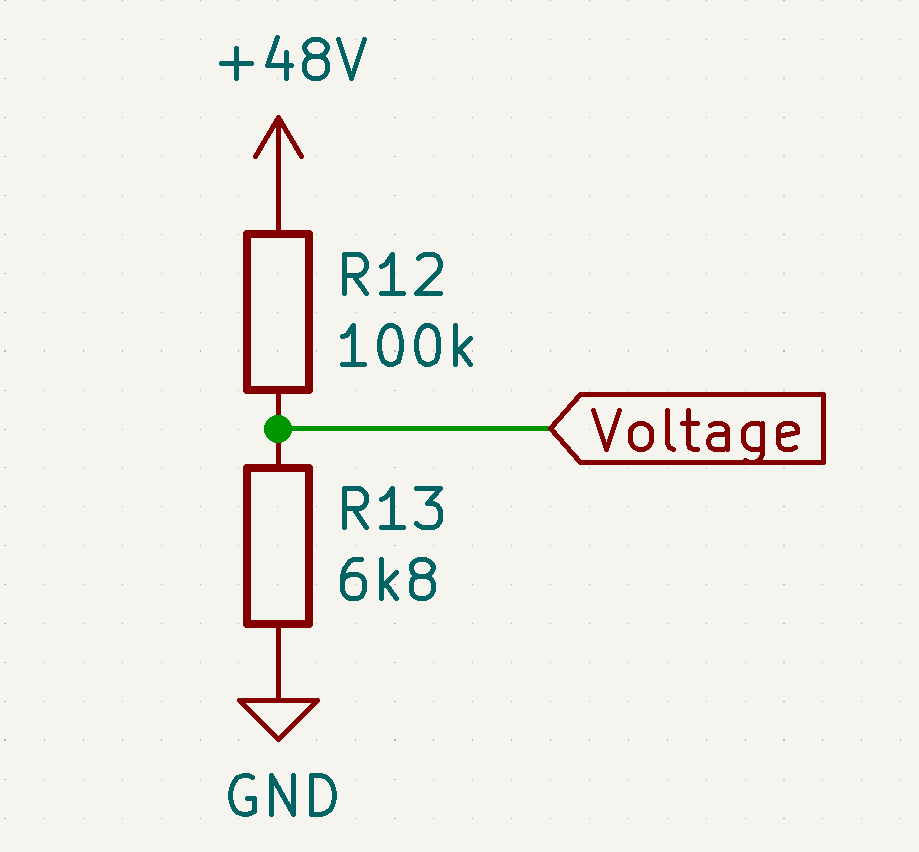
\includegraphics[scale=0.2,keepaspectratio]{assets/power-voltage.png}
    \caption{ Schematics of the powerline voltage wiring }
    \label{fig:power-voltage}
\end{figure}

Combining the formulas ($V_M = A$) we receive the following calculation in the firmware: $V = \frac{(R_1 + R_2) \cdot V_{ref}}{R_1 \cdot 2^{M}} \cdot D$.

However, the protocol specifies the data of the voltage to be in fixed format \verb|8-bit.8-bit| number, which is converted by multiplying by $255.0$ and converted to \lstinline|uint16_t|.

Each measurement and conversion is done in the \lstinline|run()| function, the results are obtained by the corresponding ``get'' function because the when the communicating through the \acrshort{spi} \acrshort{roficom} cannot measure and must provide response fast enough to the control unit.

\section[ Protocol Implementation in RoFICoM ]{ Protocol implementation in \acrshort{roficom} }
\TODOLIST{
\begin{itemize}
    \item Added power information - connection of INT and EXT, current and voltage of INT and EXT.
    \item Connection to mating side.
    \item Lidar status and distance and setting \TODO{ distance mode ?? }.
\end{itemize}
}

As previously mentioned in the \autoref{sec:roficom-firmware}, the prototype version of the firmware was missing the full implementation of the connector-to-module communication. The unfinished command is the status command, which only implemented expanding and retracting the connector based on the received command and responding with blobs remaining to be sent and received. This section describes finishing the implementation of the status command.

The function \lstinline|onCmdStatus()| accomplishes the status command parsing, reacting and responding, which is part of the reaction callback function given for the \lstinline|spiInterface|. The \lstinline|onCmdStatus()| parameters needed to be extended by the \lstinline|ConnectorStatus| (manages connection to mating connector), \lstinline|PowerSwitch| (power management), \lstinline|Lidar| and \lstinline|std::optional< LidarResult >|. The \acrshort{lidar} result is optional since the command status can be received before the \acrshort{lidar} responds with the first measurement or when the \acrshort{lidar} is not plugged in. Because of the new addition to the protocol, the structure containing the flags for command status was extended correspondingly (with \acrshort{lidar} distance mode and result status).

The \lstinline|onCmdStatus()| function can be virtually split into two halves --- the first half parses the requested command and reacts to it, while the second half creates and sends the response. The interesting part in the first half is that the \acrshort{lidar} distance mode can contain an invalid value (\lstinline|0b11|), which is simply ignored because the user's request should not be able to break the firmware.

The most interesting part of the second half is the \TODO{transformation} of \acrshort{lidar} status into the protocol flag. The values of the flag are specified in the \autoref{sec:rofi-hal-interface}. Each possible value for the flag can be derived from the possible value of \lstinline|std::optional< LidarResult >|. If the optional does not contain a value,  the result is \emph{not yet measured} (or the \acrshort{lidar} is not plugged in). Otherwise, the \lstinline|Result| class must be present. If the \lstinline|Result| has the error type set, the flag is set as such (the error value). The two checks handle the validity bit of the flag. After that, the \lstinline|Result| must contain the value type, which is the \gls{vl53l1x} result structure described in \autoref{sec:lidar-result}. The certainty bit is decided by the value of the \gls{vl53l1x} status from the result structure --- value of $0$ (i.e., the previously mentioned value of valid status) results in Fully Valid flag. In contrast, other values result in the Out of Range flag since the measurement may not be correct. Consequently, the distance is set only if the validity bit is set to valid.

\section{ Changes to the Build System }
\TODOLIST{
\begin{itemize}
    \item static buffer vs ram
    \item Hard fault = ram had too high static usage, minimizing the usage by lower the number of available buckets for packets solved this (memory::pool)
\end{itemize}
}

During the development, the firmware started hard faulting on the \acrshort{roficom}. Hard faults are exceptions that are typically caused by unrecoverable system errors. Such errors can be an execution of an Undefined instruction, an attempted load or store to an unaligned address, and many more, which are described in more detail in the ARM Devices Generic User Guide. In the debug build of prototype version the static usage of the RAM was very high (around $70\%$), not leaving enough RAM for the runtime of the firmware, which resulted in in corrupted stack frames. The fix to this issue was reducing the size of statically allocated packet buffer. The count of 1025B buffers was reduced from count of 20 to 5, bringing the static usage of RAM to manageable $30\%$.

Compiler flags \lstinline|-fstack-protector-all| and \lstinline|-fstack-check| were added to the debug build to detect similar issues as soon as possible.

\chapter[ RoFI Hardware Abstraction Layer ]{ \acrshort{rofi} \acrlong{hal} } \label{ch:rofi-hal}

This chapter describes changes made to the prototype version of the \acrshort{rofi} \acrshort{hal} --- in both: the interface and the \gls{universal-module} implementation. The \acrshort{rofi} \acrshort{hal} has been introduced in \autoref{sec:rofi-hal-desc}.

\section{Interface} \label{sec:rofi-hal-interface}

\TODOLIST{
\begin{itemize}
    \item Current interface components - RoFI, joint, connector
    \item \textbf{Proxy} 
    \item Changes done --- Added distance and status
\end{itemize}
}

The header file for the interface is in file \path{RoFI/softwareComponents/rofiHalInc/include/rofi_hal.hpp}.

The prototype version of the interface has all components as a \emph{Proxy}. Proxy object is meant to be an abstraction that does not hold the ownership of the underlying component and is meant to be lightweight, safely copyable and shareable.

The prototype version contains three main components --- \lstinline[breakatwhitespace]|RoFI|, \lstinline|Joint| and \lstinline|Connector|. The \lstinline|RoFI| represents the \acrshort{rofi} module, this object does not have a constructor and is instead received with \lstinline|RoFI::getLocalRoFI()| static method or \lstinline|RoFI::getRemoteRoFI(Id remoteId)|. Each module has its shape, consisting of the number of joints and connectors. The \lstinline|RoFI| allows to get the proxy for the module's joints and connectors. The \lstinline|Joint| proxy allows for both control and \TODO{getting joint information}.

The connector was the only component that needed a change due to the \acrshort{lidar} addition. The \lstinline|Connector| proxy has the ability to extend and retract the connector, connect and disconnect powerlines (internal or external), react to connection and disconnection from the mating side and powerlines, and send and react to received packets. The part of the \lstinline|Connector| that needed change was the \lstinline|ConnectorState|. The prototype version of the \lstinline|ConnectorState| contains information about the connector's position (extended or retracted), connection on powerlines and to the mating side, the orientation of the connection (North, East, South, West), and the voltage and current of the powerlines.

The state was extended by the measured distance, the measurement status and setting, and receiving distance modes. However, this is different from the \acrshort{lidar} status from \autoref{sec:lidar-result}. Whereas, the measured distance is just a 16-bit number with the measured distance in millimeters, the status is more complicated.

The status is a 2-bit number, with each value having assigned a specific meaning. The status values and their meanings are the following:
\begin{itemize}
    \item \lstinline|0b00| = Error --- This signals an error, which can be an \acrshort{i2c} communication error, a \acrshort{lidar} error, or that the device got unplugged while communicating.  
    \item \lstinline|0b01| = Not Measured --- This status is when the \acrshort{lidar} is not plugged in or the request was made before the first \acrshort{lidar} measurement was completed.
    \item \lstinline|0b10| = Out of Range --- The measured data was measured; however, they \textbf{does not have to be valid}. Usually, this means that the data are outside of the measurable range; however, it can also be caused by wrong settings.
    \item \lstinline|0b11| = Fully Valid --- The measured distance is fully valid to use.
\end{itemize}

The value for the Error was chosen carefully to prevent false signaling of the measured state --- if there is an error in communication with the \acrshort{roficom}, the read value is $0$, and thus the \acrshort{lidar} status is parsed as an Error. Additionally, the specific choice of values allows for the individual bits of the status to carry their own meaning, i.e., the higher bit acts as a \emph{validity} bit (the value \verb|1| means the measured data can be used). The lower bit acts as a \emph{certainty} bit (the value of \verb|1| means that the measured distance should be correct). Note that the bit can be used as a certainty bit only when the validity bit is set to valid. The \acrshort{lidar} status is for explicitness represented as a \lstinline|enum|.

The distance mode is represented as a 2-bit number, and the values correspond to the value of the distance modes for the \acrshort{lidar} driver. The possible modes for the distance mode are autonomous (with the value of $0$), short ($1$) and long ($2$). The last possible value ($3$) is currently unspecified and its usage is ignored. There a was newly added function to set the distance mode for the connector, which takes an \lstinline|enum class| of the possible modes.

\section{ Implementation --- esp32 }
\TODOLIST{
\begin{itemize}
    \item Apply changes from interface --- lidar status, distance and \TODO{distance modes}
    \item Issue $\rightarrow$ status is not being updated $\rightarrow$ Needed to implement poller
\end{itemize}
}

Since the protocol changed, the changes must be synchronized to all implementations. Not only does the protocol change need to be replaced in all of the \acrshort{rofi} \acrshort{hal} implementations, but also in the firmware implementation. The change of firmware implementation that sends the \acrshort{lidar} status, measured distance, and distance mode is described in \autoref{sec:lidar-result}. This section describes changes made in the esp32 \acrshort{hal} implementation (for the \gls{universal-module}). \TODO{Other implementations are out of the scope of this thesis.}

The prototype version has a lot of functionality implemented. Before mentioning the specific changes made, there is a short overview of how the esp32 \acrshort{hal} handles the connector-to-module communication. The \lstinline|ConnectorBus| handles any command (such as to connect and disconnect) for the local connector. The connector schedules the command to be sent over the bus. The \lstinline|ConnectorBus| for sending the commands runs on a parallel thread. The sent is handled by the function \lstinline|run()| with specified command as an argument. After the command is sent and the response is received, it is returned to the connector under the function call \lstinline|finish()|. The parsing of the response into the \lstinline|ConnectorState| is done with the function \lstinline|ConnectorStateImpl::from()|.

The changes to the esp32 implementation include new protocol flags --- (\acrshort{lidar} status) and distance modes. This is followed by parsing the status command response from the connector in the \lstinline|ConnectorStateImpl::from()|, that containing the \acrshort{lidar} status, measured distance and distance mode. The function to set the distance mode sends the status command with flags set accordingly to the chosen value. As last, due to the change in the size of the command, the change needs to be updated in the \lstinline|ConnectorBus::run()|, but also in the DMA buffer allocation of the \lstinline|ConnectorBus|.

Those changes are enough to get the status and distance. However, the state is only updated when the status command is issued; this means that the state of status and distance does not represent the current value. Updating the state was solved with the poller. This poller runs in a separate thread and periodically asks the \acrshort{roficom} to update the state. There must be a slight delay between commands to allow the \acrshort{roficom} to apply the commands and send the response. The poller is done by the FreeRTOS function \lstinline|xTaskCreate()|, which creates the new thread for polling and constantly issues the command status.

\chapter{Conclusion}

This thesis introduces changes and improvements made to the \acrshort{roficom}'s firmware prototype, making it closer to the production-ready state.

These changes consists of distance measurement using the \acrshort{lidar} and making abstraction around the specific \gls{vl53l1x} for easier usage in the firmware. The \gls{vl53l1x} required \acrshort{i2c} protocol, which was explained and implemented together with some family-specific code in the \verb|stm32cxx| drivers.

The \acrlong{bsp} has been added to isolate board-specific code and allow easier transition in different \acrshort{roficom}'s board versions.

Followed by smaller, but not less important additions to the \acrshort{roficom}'s firmware, such as new motor driver, implementation for power management and power measuring.

Lastly, this thesis described the update of connector-to-module communication to transfer the status of \acrshort{lidar}'s measurement and measured distance and allow for setting the \acrshort{lidar}'s distance mode. This change was added to the \acrshort{roficom}'s firmware, \acrshort{rofi} \acrshort{hal}'s interface and esp32 implementation for the \gls{universal-module}.

Even though many functionality works as intended, such as the \acrshort{lidar} measurement, its propagation to the \gls{universal-module}'s control unit, transition to new board version with \acrlong{bsp}, update of the connector-to-module protocol, there is still room for improvement.

Such improvement might be in the motor driver or in the power management. Even though both are implemented, they do not work as intended. The motor movement occasionally moves the gearing beyond the specified position and the magnetic sensors, which prevents the motor from moving back. The power management currently does not measure the correct values, although the formula is correct, and should be further inspect it to find the issue.

The final implement can be found in the github repository of the \acrshort{rofi} project at the address: \url{https://github.com/paradise-fi/RoFI}. The snapshot of the whole \acrshort{rofi} project containing the changes made during the development can be found in the thesis attachment. \TODO{appendix}

\appendix %% Start the appendices.
\chapter{An appendix}



\TODOLIST{
\begin{itemize}
    \item Setup project --- dev env = docker
    \item source setup.sh $\rightarrow$ compile roficom, compile hal example
    \item flashing roficom
    \item flashing esp32
\end{itemize}
}

\end{document}
